\documentclass[11pt,a4paper]{article}
\usepackage[margin=2.4cm]{geometry}
\usepackage[T1]{fontenc}
\usepackage[utf8]{inputenc}
\usepackage{lmodern,microtype}
\usepackage{amsmath,amssymb,bm}
\usepackage{booktabs,graphicx,caption,float}
\usepackage[hidelinks]{hyperref}
\usepackage{fancyhdr}
\usepackage{enumitem}
\captionsetup{font=small,labelfont=bf}
\setlist{itemsep=2pt,topsep=3pt}
\graphicspath{{figures/}}
\pagestyle{fancy}\fancyhf{}
\fancyhead[L]{\small Uncertainty-aware multimodal perception for manipulation}
\fancyhead[R]{\small \textbf{Simulation only}}
\fancyfoot[C]{\thepage}

\newcommand{\simonly}{\textbf{simulation-only}}
\newcommand{\vect}[1]{\bm{#1}}
\DeclareMathOperator{\diag}{diag}
\DeclareMathOperator{\wrap}{wrap}
\DeclareMathOperator{\tr}{tr}

\title{
    \LARGE\textbf{Uncertainty-Aware Multimodal Perception for Robotic Manipulation:}\\[4pt]
    \large\textbf{Visual, Proprioceptive and Contact Sensor Fusion under Sensor Degradation}\\[8pt]
    \large A pre-registered simulation-only study in MuJoCo
}

\author{
    Mohammed Abo Oraig\\
    \small Independent research\\
    \small\texttt{mohammed-abo-oraig@etud.univ-tln.fr}
}

\date{}

\begin{document}
\maketitle

\begin{abstract}
\noindent\textbf{All results in this report come from a simulation (MuJoCo, Franka Panda arm, one cube, one RGB camera, wrist force/torque sensor). No claim is made about real robots.}
We study per-frame estimation of a cube's pose (position and yaw) while a scripted policy picks it up, lifts it and holds it, when the vision, proprioception and contact signals are independently degraded (occlusion, noise, bias, dropouts, illumination change, \dots).
We compare vision-only, kinematic, classical weighted-least-squares and learned fusion models with an uncertainty-aware fusion model (F-CI) in which every modality is an expert that outputs its own full-covariance Gaussian, fused in information form with covariance-intersection weights, so that no conditional independence between modality uncertainties is assumed.
Three hypotheses (H1--H3) and their decision rules were fixed in a pre-registration \emph{before} the test split was used.
On the test split, with three training seeds and paired episode-level bootstrap statistics with Holm correction:
\textbf{H1 is supported} (fusion lowers the xy error against vision-only by 2.3--44.7\,mm under occlusion, but also by 2.0\,mm on clean data, so the gain is only weakly ``particular'' to occlusion, and fusion is \emph{worse} than vision-only under occlusion combined with a constant proprioceptive bias);
\textbf{H2 is supported} (F-CI has lower NLL than both non-uncertainty-aware fusion baselines in 9/9 failure scenarios, and is the best calibrated of three fusion rules);
\textbf{H3 is only partially supported} (mixed-degradation training greatly improves NLL on unseen failure combinations, but does not reach the performance of a model that saw those combinations; the benefit is mostly calibration, not accuracy).
Several development-time leaks that would have inflated the results were found and removed; they are documented in Section~\ref{sec:leaks}.
\end{abstract}

\tableofcontents
\clearpage

%==============================================================================
\section{Introduction and scope}
A manipulation system rarely has a single reliable sensor. Cameras are occluded by the arm or by objects, joint encoders can be noisy or biased, and force sensing is only informative once the hand touches something. A perception module that fuses these streams should (i) be more accurate than any single stream, (ii) know \emph{how} wrong it may be, and (iii) degrade gracefully when one stream becomes unreliable.

This project asks whether \emph{explicit per-modality uncertainty} helps for this purpose, in a deliberately small, fully controlled setting. Everything is \simonly: one Franka Panda in MuJoCo~\cite{todorov2012mujoco} (model from MuJoCo Menagerie~\cite{menagerie}), one cube, one RGB camera, joint positions and velocities, and a wrist force/torque sensor. We use PyTorch and Python. We do \emph{not} use ROS~2, reinforcement learning, motion planning beyond a scripted policy, multiple objects, or sim-to-real transfer.

\paragraph{Hypotheses.} Fixed by the project brief:
\begin{description}[leftmargin=2.2em,labelwidth=2em]
\item[H1] Multimodal fusion improves object-state estimation compared with vision-only perception, particularly under visual occlusion.
\item[H2] Explicit uncertainty estimation improves fusion reliability when individual modalities become unreliable.
\item[H3] Training with controlled sensor degradation improves generalisation to previously unseen combinations of sensor failures.
\end{description}
The experiments were designed so that each could be disproved. Operational decision rules (Section~\ref{sec:prereg}) were frozen on 2026-11-23 (SHA-256 of the pre-registration file: \texttt{DDD7509465C4\dots4513BFBAA}, full hash in Appendix~B and in \texttt{docs/FREEZE.txt}) before the test split was evaluated.

\paragraph{Contributions.}
(1) A reproducible simulation, data-generation and degradation framework with episode-level splits; (2) a mathematically specified heteroscedastic full-covariance Gaussian loss and an uncertainty-aware fusion network with three fusion rules, one of which (covariance intersection) is consistent under any unknown correlation between experts; (3) a pre-registered evaluation with paired statistics and multiple seeds; (4) a candid account of what did \emph{not} work and of the information leaks we found along the way.

%==============================================================================
\section{Problem setting}
\subsection{Task, sensors and state}
A scripted controller moves the Panda above a cube lying on a table at a random position, descends, closes the gripper, lifts the cube and holds it. Episodes last about 8.3\,s and are logged at 20\,Hz (166 frames on average). The cube (4\,cm edge, 0.2\,kg) is placed uniformly in $x\in[0.40,0.60]$\,m, $y\in[-0.20,0.20]$\,m with random yaw.

The estimator receives, at each frame: a $96{\times}96$ RGB image from a fixed camera; the seven arm joint positions and velocities and the finger opening; and the six-component wrist force/torque. It outputs an estimate of the state
\begin{equation}
\vect y = [x,\,y,\,z,\,\varphi]^\top,\qquad \varphi = 4\,\psi \pmod{2\pi},
\end{equation}
where $\psi$ is the yaw. The cube is square, so yaw is only identifiable modulo $90^\circ$; the factor 4 maps this ambiguity to a single point of the circle, so that a regression target exists. Orientation error is reported as yaw error in degrees on the quotient (chance level $22.5^\circ$).

\subsection{What is observable, and when}
\label{sec:stages}
Each frame is assigned to one of five stages: \texttt{free} (hand far from the cube), \texttt{hover}, \texttt{grasp}, \texttt{coupled} (cube lifted and held) and \texttt{post}. Proprioception tells where the \emph{hand} is. It reveals the cube only when the cube is rigidly attached to the hand, so the proprioceptive expert is \emph{gated} to the holding phase. Without that gate a per-frame model can exploit the scripted policy (the hand hovers exactly above the cube) and appear to ``measure'' the cube from joint angles; we observed this and removed it (Section~\ref{sec:leaks}). Contact (wrench) is informative only during the grasp and hold, and is conditioned on the proprioceptive features, because a wrench alone does not locate the cube in the world.

Consequently, \textbf{the only stage in which all three modalities carry information about the cube is \texttt{coupled}}, and this is the stage on which all pre-registered decisions are made. Other stages are reported as secondary; in stages where nothing is observable the best possible estimate is the prior, and models are expected to be calibrated rather than accurate there.

\subsection{Degradations}
\label{sec:degradations}
Twelve degradation families are implemented, each with levels 0 (identity) to 4 and calibrated physical units (Table~\ref{tab:families}): occlusion by a grey square on the cube (with two decoy squares so that the square's position does not reveal the cube), random-rectangle occlusion, image noise, blur, illumination gain/gamma, vision dropout (black frames in bursts), proprioceptive noise, bias with drift, bursty dropout, and the same three for contact. Dropouts are Markov bursts with a mean length of 5 frames (0.25\,s). All degradations are generated by a stateless random generator keyed by (seed, scenario, episode), so every model sees identical corrupted data.

\begin{table}[t]
\centering\small
\begin{tabular}{llc}
\toprule
Family & Unit of the level & Level 1 $\to$ 4\\
\midrule
occlusion (targeted) & square side / apparent cube width & 0.5 $\to$ 2.0\\
occlusion (random) & image area fraction & 0.10 $\to$ 0.75\\
image noise & grey levels (of 255) & 5 $\to$ 40\\
blur & Gaussian $\sigma$, px & 0.5 $\to$ 2.5\\
illumination & gain range $a$ & 0.15 $\to$ 0.80\\
vision dropout & drop probability & 0.05 $\to$ 0.40\\
proprio noise & joint-angle $\sigma$, rad & 0.002 $\to$ 0.020\\
proprio bias (+drift) & joint-angle offset $\sigma$, rad & 0.005 $\to$ 0.040\\
proprio dropout & drop probability & 0.05 $\to$ 0.40\\
contact noise / bias / dropout & force $\sigma$ N (torque: $0.05\,\mathrm{m}\times$) & 0.1 $\to$ 1.0\\
\bottomrule
\end{tabular}
\caption{Degradation families (all simulated). Torque noise is derived from the force noise through a fixed 5\,cm moment arm.}
\label{tab:families}
\end{table}

\paragraph{Evaluation scenarios.} Sixteen scenarios are evaluated on every split: clean; single-family degradations at level 2--4 (listed in the tables); one two-family failure (vision dropout L4 with proprioceptive dropout L3, where nothing is observable); and two \emph{unseen combinations} used for H3: \emph{occlusion L3 + proprio noise L2} and \emph{occlusion L4 + proprio bias L3}.

\paragraph{Mixed-degradation training.} In mixed training the training set is re-degraded every two epochs: an episode stays clean with probability 0.15; otherwise each relevant family is independently active with probability 0.3 at a random level 1--4. The pairs (occlusion, proprio noise) and (occlusion, proprio bias) are \emph{forbidden}: they are never active together in training. Model selection uses a fixed degraded validation set.

%==============================================================================
\section{Methods}
\subsection{Heteroscedastic Gaussian NLL with a positive-definite covariance}
\label{sec:nll}
For an input $\vect x$ the network outputs a mean $\hat{\vect y}=[\hat{\vect p},\hat\varphi]$ and a lower-triangular factor $\vect L(\vect x)\in\mathbb R^{4\times4}$ with
\begin{equation}
l_{ii}=\operatorname{softplus}(a_{ii})+\epsilon,\qquad l_{ij}\ (i>j)\ \text{unconstrained},\qquad \vect\Sigma=\vect L\vect L^\top,
\end{equation}
so $\vect\Sigma\succ 0$ for any network output ($\epsilon=10^{-3}$). The covariance is a \emph{full} $4{\times}4$ matrix: position--yaw and inter-axis cross-covariances are learned, and no independence is assumed. Position outputs are affine in the training mean/standard deviation, and the covariance is expressed in metres. With the tangent-space error
\begin{equation}
\vect e=\begin{bmatrix}\vect p-\hat{\vect p}\\ \wrap(\varphi-\hat\varphi)\end{bmatrix},\qquad \vect z=\vect L^{-1}\vect e\ \text{(triangular solve)},
\end{equation}
the negative log-likelihood is
\begin{equation}
\mathrm{NLL}(\vect x,\vect y)=\tfrac12\,\vect z^\top\vect z+\sum_{i=1}^4\log l_{ii}+2\log 2\pi
=\tfrac12\vect e^\top\vect\Sigma^{-1}\vect e+\tfrac12\log\det\vect\Sigma+2\log 2\pi .
\label{eq:nll}
\end{equation}
\paragraph{Properties and pitfalls (derived before implementation).}
The gradient with respect to the mean is $-\vect\Sigma^{-1}\vect e$: a large predicted variance switches off learning of the mean, so a model can ``explain away'' a bad fit; we observed that the NLL alone does not fit the mean from scratch. We therefore use an MSE warm-up on the normalised tangent error (3 epochs) during which the covariance is already trained with weight 0.1 through the NLL on a \emph{detached} mean; this removed loss spikes of up to $10^{9}$ at the switch. Over a flexible Gaussian family the population minimiser is the conditional mean and covariance of $\vect y\mid\vect x$, so a calibrated model has $\mathbb E[d^2]=4$ for $d^2=\vect e^\top\vect\Sigma^{-1}\vect e$ (4 degrees of freedom). The wrapped residual keeps the loss bounded, but a Gaussian is a crude model when yaw is unobservable. The model captures \emph{aleatoric} uncertainty only; whether it is also calibrated for unseen degradations is a measured, not assumed, property. The computation is done in fp32 even when the networks use half precision.

\subsection{Modality encoders}
\begin{itemize}
\item \textbf{Vision:} a GroupNorm CNN (width 32) with a spatial-softmax keypoint layer~\cite{finn2016deep} (32 keypoints) and global average pooling, producing a 128-D embedding.
\item \textbf{Proprioception:} an MLP (3 layers, 256 units) on standardised joint positions, velocities, forward-kinematics features of the hand and the holding gate; inputs are clamped to $\pm10$ standard deviations and missing samples are zero-filled with an explicit mask.
\item \textbf{Contact:} an MLP (3 layers, 128 units) on 13 features: wrench (6), gravity direction in the hand frame (3), TCP height, finger opening, joint-speed norm and the holding gate. It is conditioned on the proprioceptive features.
\end{itemize}
Each unimodal model attaches a Gaussian head (Section~\ref{sec:nll}). Training uses 20 epochs, batch size 128, learning rate $2\cdot10^{-3}$ (fusion models $10^{-3}$), weight decay $10^{-4}$, gradient clipping at 5, and fp16 autocast on the GPU. The checkpoint with the lowest validation NLL after warm-up is kept.

\subsection{Baselines}
\begin{description}[leftmargin=1em]
\item[Classical (no learning).] B1 colour-segmentation vision with a table-height or broad-height prior; B3/B3c forward-kinematics proprioception (with the contact residual) gated to the holding phase; B6/B6c weighted-least-squares (WLS) fusion of the two, with variances calibrated on the training split. Each is also run with the \emph{true} degradation levels given as noise variances (``oracle''), which is an upper bound for this family rather than a deployable baseline.
\item[Learned unimodal.] Vision-only and gated-proprioception networks, trained on clean data and with mixed degradations (``\emph{m}'' variants).
\item[Learned non-uncertainty-aware fusion.] \textbf{F0} concatenates the three embeddings (missing inputs zero-filled, unmasked); \textbf{F1} adds explicit availability masks; \textbf{F2} multiplies each embedding by a learned sigmoid reliability gate. Each outputs one joint Gaussian through the same head. They are \emph{not} point estimators; what they lack is a separate uncertainty per modality.
\end{description}

\subsection{Uncertainty-aware fusion}
\label{sec:uafusion}
Three experts $m\in\{$vision, proprioception, contact$\}$ each output a Gaussian $(\vect\mu_m,\vect\Sigma_m)$ with precision $\vect\Lambda_m=\vect\Sigma_m^{-1}$ (the contact expert receives the proprioceptive features). A broad Gaussian prior $(\vect\mu_0,\vect\Lambda_0)$ covers the table workspace. The fused estimate is, in information form,
\begin{equation}
\vect\Lambda=\vect\Lambda_0+\sum_m a_m\vect\Lambda_m,\qquad
\vect\Lambda\vect\mu=\vect\Lambda_0\vect\mu_0+\sum_m a_m\vect\Lambda_m\vect\mu_m,\qquad a_m=w_m\,\mathbf{1}[\text{expert }m\text{ available}].
\label{eq:fusion}
\end{equation}
The yaw coordinate is unwrapped around the precision-weighted circular mean before averaging. Three rules differ in the weights $w_m$:
\begin{itemize}
\item \textbf{PoE} ($w_m=1$): the product of experts, which is the Bayes-optimal rule \emph{if} the experts' errors are conditionally independent;
\item \textbf{tPoE} ($w_m\in(0,1)$ through a sigmoid): tempered product of experts;
\item \textbf{CI} ($w_m\ge0$, $\sum_m w_m=1$ over the available experts, through a softmax): \emph{covariance intersection}~\cite{julier1997non}. For the combination $\vect\Lambda=\sum_m w_m\vect\Lambda_m$ the fused covariance is consistent (never over-confident) \emph{whatever the unknown cross-correlation} between the experts' errors, provided each expert is itself consistent. This is the rule that does not assume conditional independence of the modality uncertainties.
\end{itemize}
The weights are produced by a small network that sees, \emph{detached}, the log-diagonal of every expert's $\vect L$, the availability masks and pairwise disagreement features $\log(1+d_{mn}^2)$. Training minimises the NLL of the fused Gaussian plus $0.5\times$ the sum of per-expert NLLs (auxiliary loss), so that each expert is individually meaningful. The guarantee for CI is conditional on calibrated experts and is an \emph{empirical} question for learned experts: Section~\ref{sec:results} measures it. The classical WLS baseline corresponds to PoE with hand-calibrated variances.

%==============================================================================
\section{Experimental protocol}
\label{sec:prereg}
\paragraph{Data and splits.} 600 training, 150 validation, 150 test and 100 \emph{test\_ood} episodes (cube starts in a region outside the training sampling range), with episode-level splits and a fixed data seed; $96{\times}96$ images. The validation split was used for every design decision; the test split was evaluated once after the freeze, test\_ood afterwards.

\paragraph{Models and seeds.} Fourteen learned models $\times$ 3 training seeds were trained with identical configuration (the protocol runner fingerprints all configuration files and refuses to continue if one changes). The set includes mixed- and clean-trained variants, the three fusion rules, and two controls: \emph{allcombos} (F-CI trained with the forbidden pairs allowed) and \emph{nocontact} (F-CI whose contact expert never has data).

\paragraph{Metrics.} xy RMSE (mm), yaw MAE ($^\circ$), NLL (Eq.~\ref{eq:nll}), mean $d^2$, and coverage of the 68\,\% and 95\,\% ellipsoids, per stage and over all frames; reliability diagrams and error-versus-predicted-$\sigma$ curves.

\paragraph{Statistics.} The unit of replication is the episode. Seeds are combined by averaging per-episode sums. Methods are compared with a \emph{paired} cluster bootstrap over episodes (5000 resamples, 95\,\% percentile intervals, one-sided $p$) and Holm--Bonferroni correction~\cite{holm1979} within each hypothesis' family of tests at $\alpha=0.05$ (bootstrap~\cite{efron1979}). Because an episode bootstrap does not capture training-seed variance, a result is called significant only if it is also in the same direction in \emph{every} seed. Differences below 1\,mm xy are not treated as practically significant. Reported $p$-values are limited by the bootstrap resolution ($1/5001$; $0.004$ after Holm for 18 tests).

\paragraph{Decision rules (frozen).}
All on the \texttt{coupled} stage of the test split.
\begin{description}[leftmargin=1em]
\item[H1] Candidate F-CI, reference vision-only (mixed-trained), xy RMSE. \emph{Supported} if (a) in $\ge2$ of 3 occlusion scenarios (occlusion L2, L4, random-rectangle L4) the gain is significant and $\ge1$\,mm, and (b) the relative gain $1-\mathrm{RMSE}_{\text{F-CI}}/\mathrm{RMSE}_{\text{vision}}$ is larger under occlusion L4 than on clean data (95\,\% CI of the contrast excluding 0). \emph{Partially supported}: (a) only. \emph{Falsified}: (a) fails or the gain is not larger under occlusion.
\item[H2] Candidate F-CI against F1 and F2 on nine single-modality failures. \emph{Supported} if for \emph{both} comparators F-CI has significantly lower NLL in $\ge6$ of 9 scenarios and is significantly less accurate (by $\ge1$\,mm) in at most 2. \emph{Falsified} if fewer than 6 NLL gains.
\item[H3] F-CI trained with mixed degradations against F-CI trained on clean data on the two unseen combinations (NLL). Control: non-inferiority of the mixed model to the \emph{allcombos} model (upper CI bound of $\Delta$NLL $\le0.5$ nats and of the RMSE ratio $\le1.25$). \emph{Supported} if both, \emph{partially} if only the first, \emph{falsified} if the first fails.
\end{description}
The pre-registration additionally recorded predictions made on the validation split, among them that fusion would \emph{not} beat vision-only under occlusion with a proprioceptive bias, and (wrongly) that the contact expert would add little; both are discussed below.

%==============================================================================
\section{Results (test split, simulation only)}
\label{sec:results}
Unless stated otherwise, numbers are mean over three training seeds on the \texttt{coupled} stage. Complete tables for all sixteen scenarios are in Appendix~\ref{app:tables}.

\begin{figure}[t]
\centering
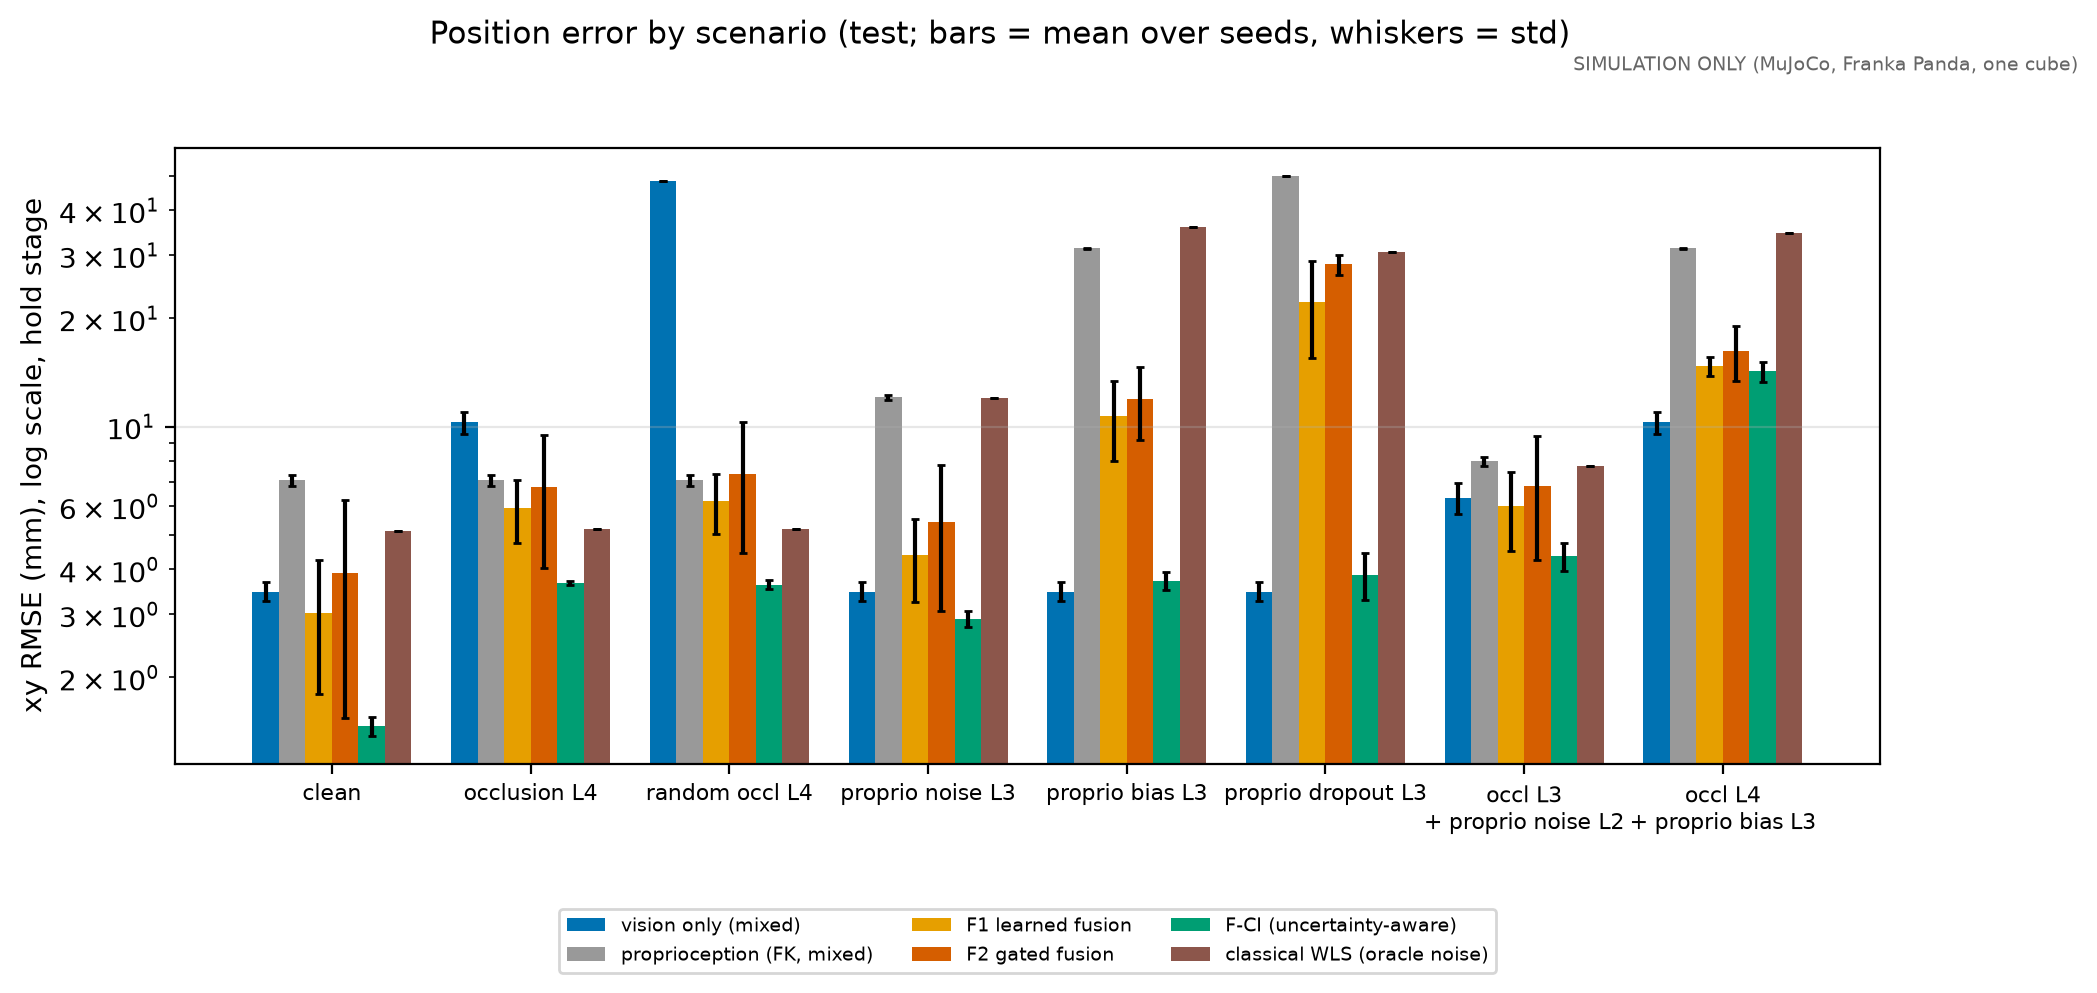
\includegraphics[width=\textwidth]{fig1_rmse_by_scenario.png}
\caption{Position error in the hold stage for selected scenarios (log scale; whiskers: standard deviation over seeds). Simulation only.}
\label{fig:rmse}
\end{figure}

\subsection{H1: fusion versus vision-only}
\begin{table}[t]\centering\small\begin{tabular}{lrrrrr}\toprule
Scenario & vision & F-CI & $\Delta$ (95\,\% CI) & $p_{\mathrm{Holm}}$ & seeds \\\midrule
occlusion L2 & 5.0 & 2.7 & $-2.3$ [-2.7,-1.9] & 0.001 & 3/3 \\
occlusion L4 & 10.3 & 3.7 & $-6.6$ [-7.2,-6.0] & 0.001 & 3/3 \\
random occl L4 & 48.4 & 3.6 & $-44.7$ [-47.3,-42.2] & 0.001 & 3/3 \\
clean$^{*}$ & 3.5 & 1.5 & $-2.0$ [-2.2,-1.8] & -- & 3/3 \\
vision dropout L3$^{*}$ & 50.5 & 2.1 & $-48.5$ [-52.5,-44.3] & -- & 3/3 \\
occl L4 {+} proprio bias L3$^{*}$ & 10.3 & 14.3 & $+4.0$ [+2.7,+5.2] & -- & 0/3 \\
\bottomrule\end{tabular}\caption{H1, test split, hold stage, xy RMSE in mm. $\Delta=$ RMSE(F-CI) $-$ RMSE(vision); negative favours fusion. Rows marked $^{*}$ are reported but not part of the decision rule. Seeds: number of training seeds in which F-CI is lower.}\label{tab:h1}\end{table}

Fusion improves on vision-only in all three occlusion scenarios (Table~\ref{tab:h1}, Fig.~\ref{fig:forest}): by 2.3\,mm (occlusion L2), 6.6\,mm (L4) and 44.7\,mm (random rectangles), each Holm-significant and consistent in all three seeds. Rule (a) holds. The relative gain is $0.64$ under occlusion L4 and $0.58$ on clean data; the contrast is $0.067$ with 95\,\% CI $[0.017,0.120]$, so rule (b) holds, \textbf{but only narrowly}: fusion is better than vision-only \emph{even when nothing is wrong} (1.5 versus 3.5\,mm), so the benefit is mostly uniform and only weakly specific to occlusion. H1 is supported under the pre-registered rule; we regard the ``particularly'' part as weak evidence.

\begin{figure}[t]
\centering
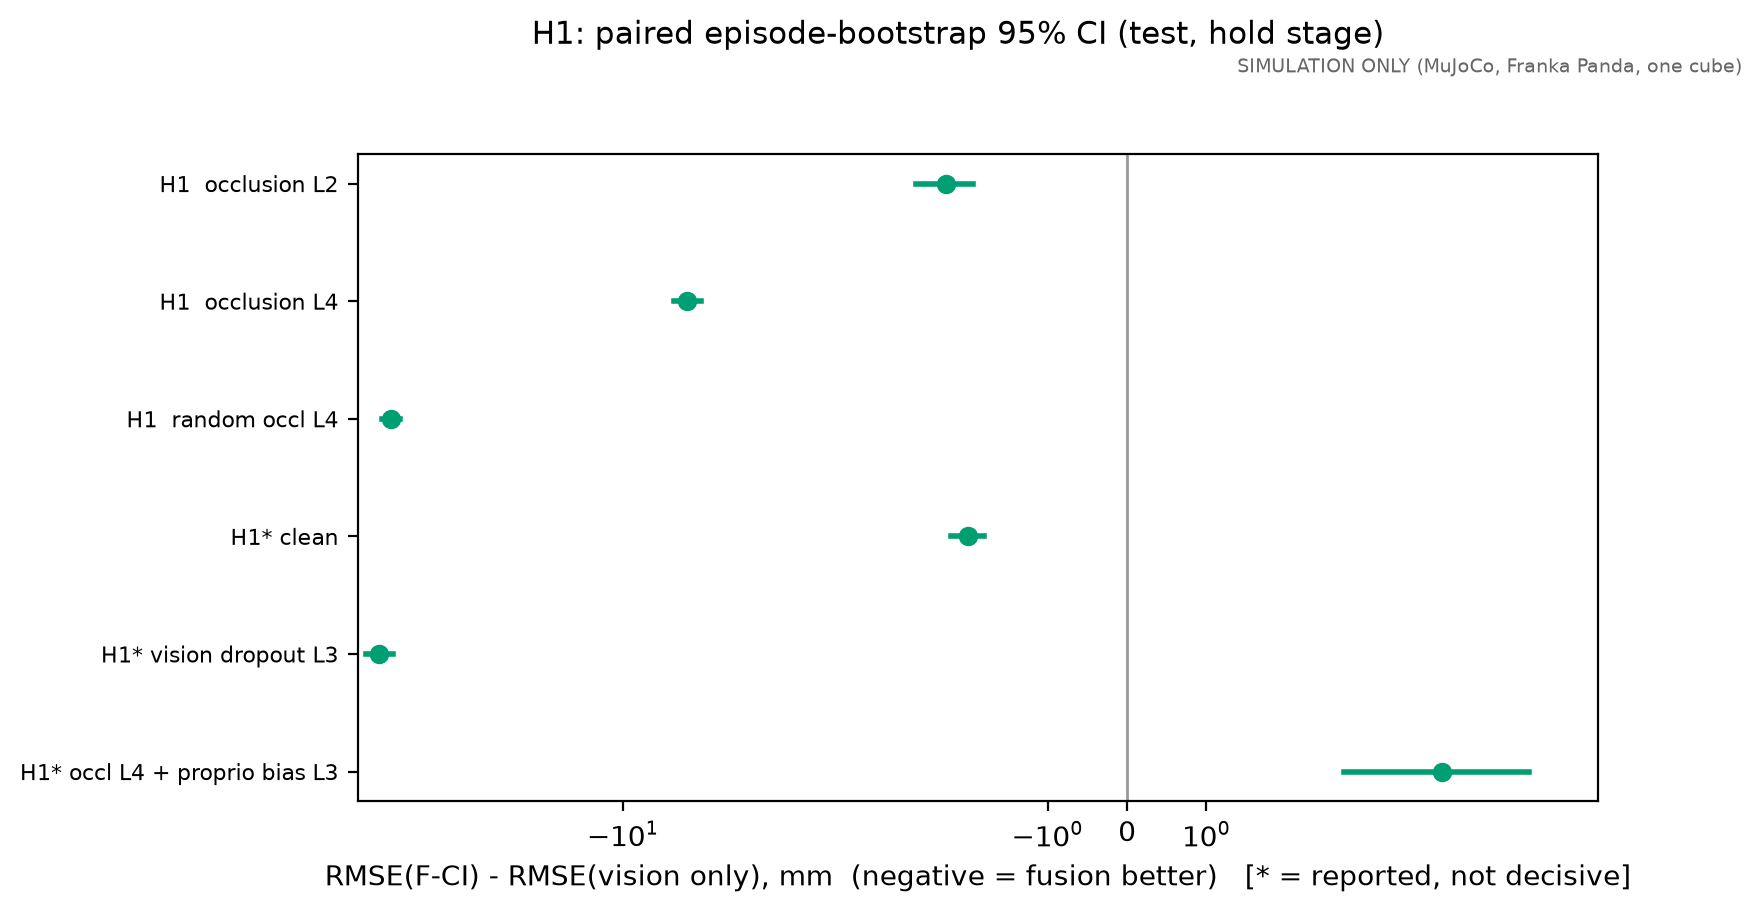
\includegraphics[width=0.78\textwidth]{fig7_h1_forest.png}
\caption{H1: difference of xy RMSE (F-CI minus vision-only) with paired bootstrap 95\,\% CI. Negative favours fusion. Rows marked H1* are reported but do not enter the decision. Simulation only.}
\label{fig:forest}
\end{figure}

\paragraph{Limits of the H1 result.}
(i) Under \emph{occlusion L4 combined with a proprioceptive bias} F-CI (14.3\,mm) is \emph{worse} than vision-only (10.3\,mm; $\Delta=+4.0$, CI $[2.7,5.2]$, worse in all seeds), as predicted on validation: a constant proprioceptive bias is not removed by fusion, it is only reported as uncertainty.
(ii) Pooled over \emph{all} frames, F-CI is slightly worse than vision-only under occlusion L4 (41.2 versus 36.2\,mm; clean: 1.2 versus 2.2\,mm). Outside the hold stage the only informative stream is vision, and the vision expert inside the fusion network is a little worse than the stand-alone vision network. The pre-registered H1 comparison is restricted to the stage where a second modality exists, which is a legitimate but favourable choice; the pooled number shows its price.
(iii) With vision entirely absent (vision dropout L3) the gain is large (2.1 versus 50.5\,mm), which is expected and uninformative about uncertainty handling.

\subsection{H2: does explicit per-modality uncertainty help?}
\begin{table}[t]\centering\small\begin{tabular}{lrrrrrr}\toprule
 & \multicolumn{3}{c}{NLL} & \multicolumn{3}{c}{xy RMSE (mm)} \\\cmidrule(lr){2-4}\cmidrule(lr){5-7}
Scenario & F-CI & F1 & F2 & F-CI & F1 & F2 \\\midrule
occlusion L4 & -16.54 & -13.43 & -13.44 & 3.7 & 6.0 & 7.3 \\
random occl L4 & -16.56 & -13.27 & -13.20 & 3.6 & 6.3 & 7.9 \\
vis noise L3 & -17.83 & -15.38 & -15.18 & 1.8 & 3.5 & 4.7 \\
illumination L3 & -18.09 & -15.54 & -15.30 & 1.7 & 3.4 & 4.7 \\
blur L3 & -18.23 & -15.58 & -15.38 & 1.5 & 3.3 & 4.5 \\
vision dropout L3 & -18.03 & -15.18 & -14.95 & 2.1 & 4.2 & 5.5 \\
proprio noise L3 & -16.01 & -14.31 & -14.03 & 2.9 & 4.5 & 5.9 \\
proprio bias L3 & -15.89 & -12.35 & -12.38 & 3.7 & 11.1 & 12.2 \\
proprio dropout L3 & -17.54 & -13.73 & -13.23 & 3.9 & 23.2 & 28.3 \\
\bottomrule\end{tabular}\caption{H2, test split, hold stage. F-CI has a significantly lower NLL than both non-uncertainty-aware fusions in all 9 scenarios (all Holm-adjusted $p=0.004$, the floor of the 5000-resample bootstrap after Holm for 18 tests; all 3 seeds agree) and is never significantly less accurate.}\label{tab:h2}\end{table}

In all nine single-modality failure scenarios F-CI has a significantly lower NLL than both non-uncertainty-aware fusion models, with all three seeds agreeing, and it is never significantly less accurate; in most scenarios it is also more accurate (Table~\ref{tab:h2}). The largest accuracy differences occur when proprioception fails: with proprioceptive dropout F-CI reaches 3.9\,mm whereas F1 and F2 reach 23.2 and 28.3\,mm, since the monolithic networks cannot fall back on the healthy modality. H2 is supported.

\paragraph{Calibration.}
Fig.~\ref{fig:calib} shows reliability diagrams pooled over the failure set. On single failures (left) F-CI lies closest to the diagonal, slightly conservative at low nominal levels. On the unseen combinations (right) F-CI and the vision-only model are the best calibrated, both mildly over-confident at the 95\,\% level, while F1, the product of experts and especially the clean-trained model are strongly over-confident (the clean-trained model's coverage is essentially zero). Numerically (Tables~\ref{tab:app_cov} and~\ref{tab:app_d2}), the 95\,\% coverage over the single-failure scenarios is 0.86--0.98 for F-CI, 0.62--0.80 for the product of experts and 0.76--0.88 for the tempered variant; on the two combinations it is 0.82 for F-CI against 0.52 and 0.61 (PoE). Mean $d^2$ of F-CI is 3.1--5.6 on single failures (target 4) and 6.2 and 7.2 on the two combinations. The model trained on clean data is catastrophically over-confident under proprioceptive faults (mean $d^2$ of $2\cdot10^{4}$ for noise and $2\cdot10^{6}$ for bias).

\begin{figure}[t]
\centering
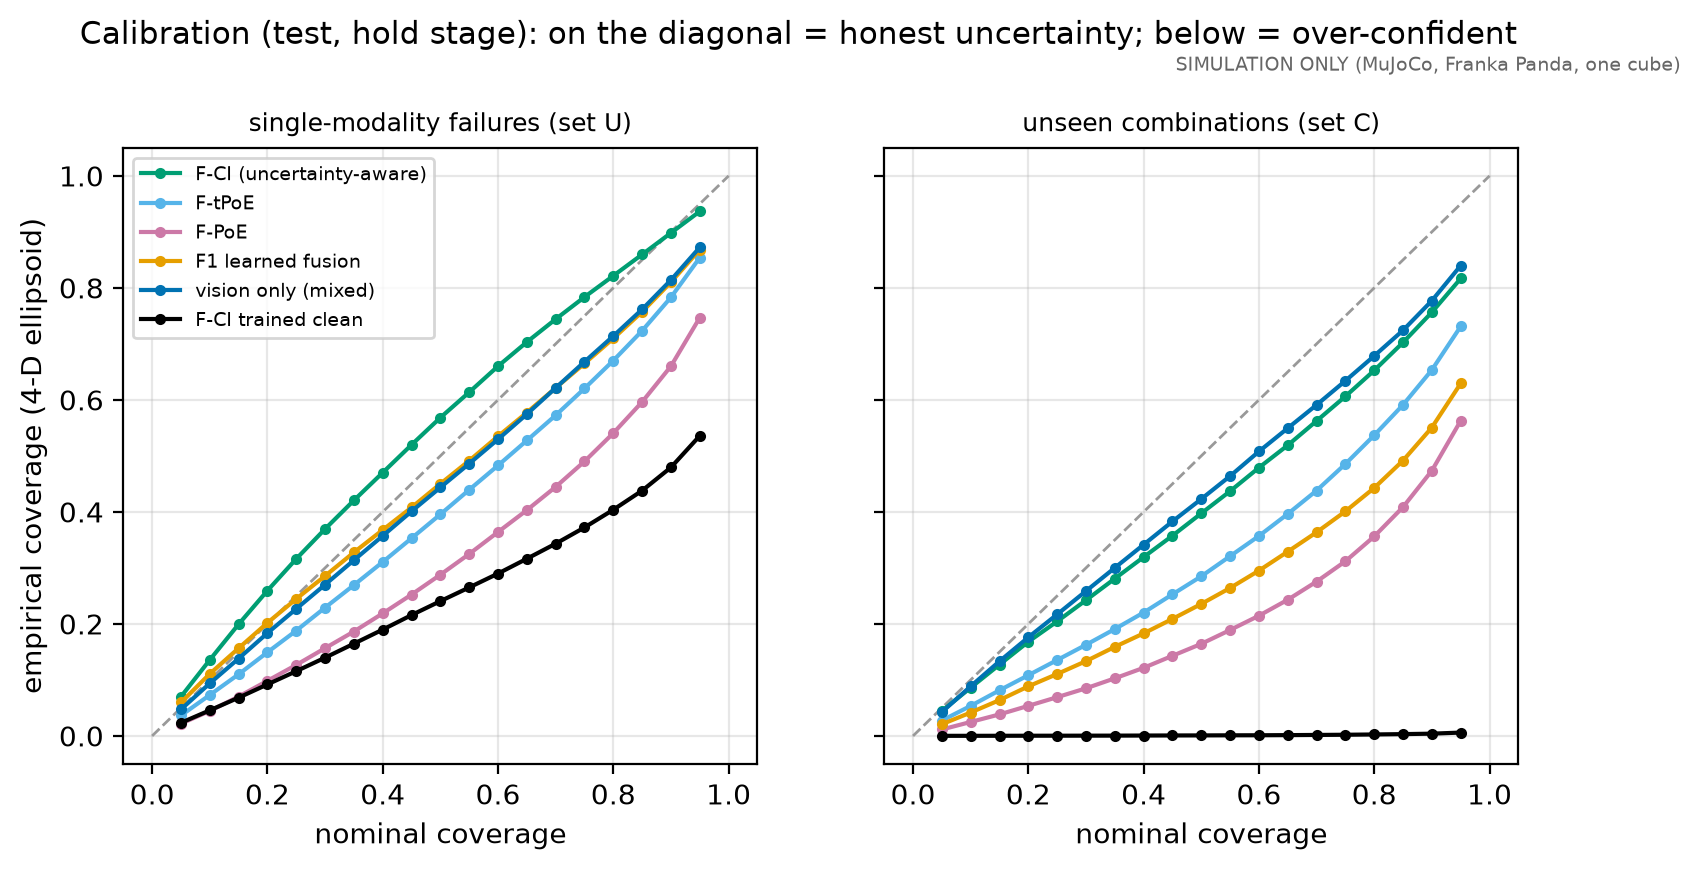
\includegraphics[width=\textwidth]{fig2_reliability.png}
\caption{Reliability of the predicted 4-D uncertainty ellipsoids in the hold stage, pooled over single-modality failures (left) and the two unseen combinations (right). Below the diagonal means over-confident. Simulation only.}
\label{fig:calib}
\end{figure}

\paragraph{Does the independence assumption matter? (H2b)}
Across the nine failure scenarios, F-CI's calibration gap $|d^2-4|$ is smaller than that of the product of experts and of the tempered variant in 9/9 scenarios (mean gap 0.60 against 4.35 and 1.66). F-CI also has lower NLL than PoE in 9/9 scenarios, but only in 4/9 against tPoE, with differences of at most 0.24 nats in magnitude. So CI mostly buys calibration, not accuracy; PoE's independence assumption demonstrably costs both when experts are correlated.

\paragraph{Error versus predicted uncertainty.}
In Fig.~\ref{fig:sigma} the realised error of F-CI tracks the predicted $\sigma$ along the diagonal over the range where data exist (0.5--8\,mm). The learned fusion F1 under-predicts its error at predicted $\sigma\gtrsim 12$\,mm by up to a factor of two. The uncertainty is useful for ranking frames by expected error, not only on average.

\begin{figure}[t]
\centering
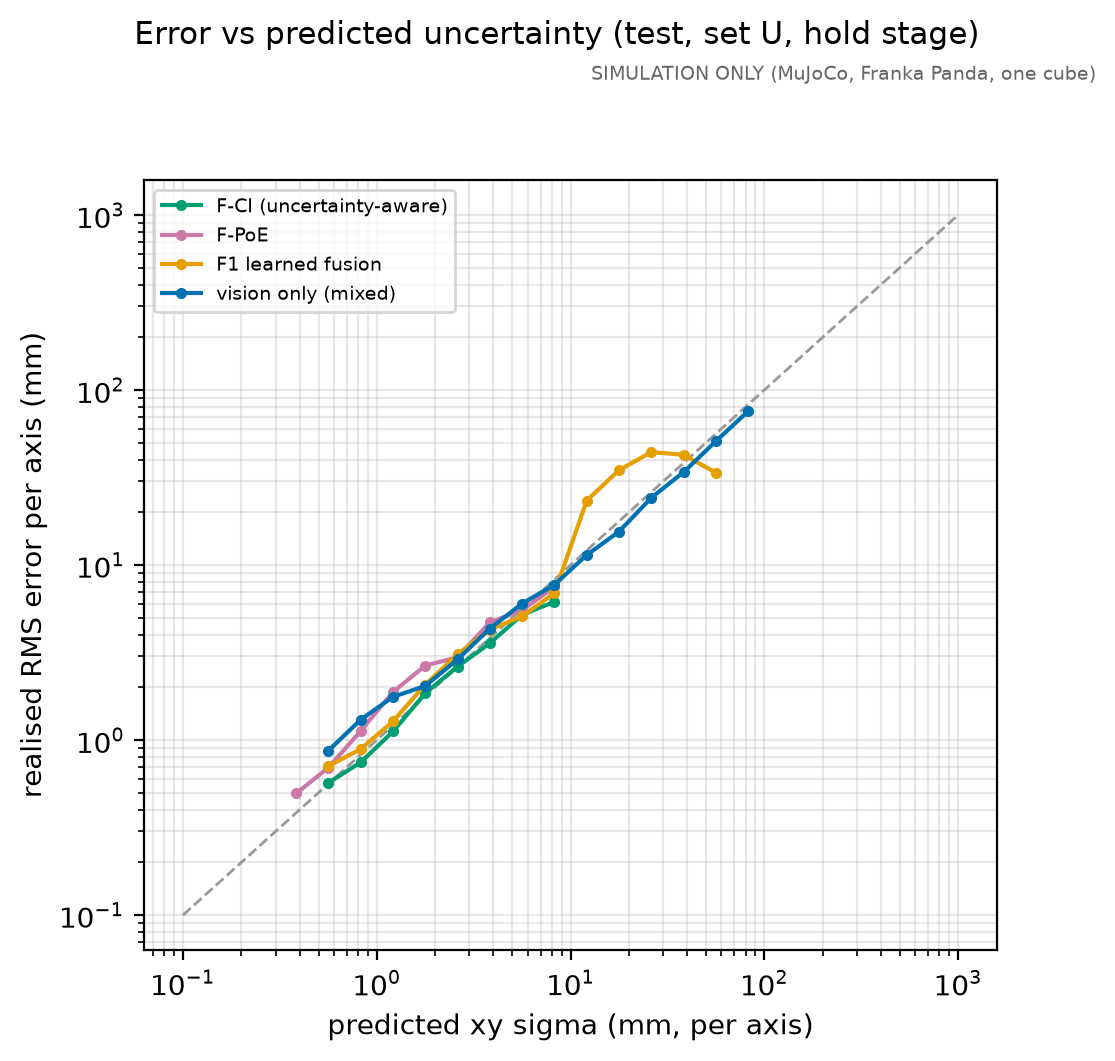
\includegraphics[width=0.62\textwidth]{fig3_error_vs_sigma.png}
\caption{Realised RMS error per axis versus predicted standard deviation (bins with at least 200 frames; hold stage; failure set). Simulation only.}
\label{fig:sigma}
\end{figure}

\paragraph{Comparison with classical fusion (H2c).}
Even when the classical WLS fusion is given the \emph{true} noise levels (oracle), F-CI has lower xy RMSE in all nine scenarios, by 1.5\,mm (occlusion) to 32\,mm (proprioceptive bias). With calibrated but non-oracle variances (B6), the classical NLL explodes under proprioceptive faults (25.6 for noise, 146.1 for bias, compared with $-16$ for F-CI). This does not show that classical fusion is poor in general: its inputs here are hand-designed colour segmentation and kinematics, which are much cruder than the learned experts.

\subsection{H3: training with degradation and unseen combinations}
\begin{table}[t]\centering\small\begin{tabular}{lrrr}\toprule
Scenario (unseen combination) & mixed & clean-trained & seen-combination control \\\midrule
occl L3 {+} proprio noise L2 (NLL) & -14.44 & $160.4$ & -15.14 \\
occl L4 {+} proprio bias L3 (NLL) & -10.33 & $1.1\!\times\!10^{6}$ & -11.23 \\
\midrule
occl L3 {+} proprio noise L2 (RMSE, mm) & $4.3{\pm}0.4$ & $5.0{\pm}0.1$ & $3.6{\pm}0.1$ \\
occl L4 {+} proprio bias L3 (RMSE, mm) & $14.2{\pm}0.9$ & $24.0{\pm}2.7$ & $11.4{\pm}0.2$ \\
\bottomrule\end{tabular}\caption{H3, test split, hold stage. The two scenarios combine occlusion with a proprioceptive fault that never co-occurred in mixed training; the control model was trained with these combinations allowed. NLL differences between mixed and clean-trained models are significant after Holm correction in both scenarios (Fig.~\ref{fig:matrix}); the non-inferiority margins (0.5 nats, RMSE ratio 1.25) are not met in either scenario.}\label{tab:h3}\end{table}

Mixed-degradation training lowers the NLL on both unseen combinations from $+160$ and $+1.1\cdot10^{6}$ to $-14.4$ and $-10.3$ (Holm $p<0.001$, all seeds), see Table~\ref{tab:h3} and Fig.~\ref{fig:matrix}. The \emph{accuracy} gain is much smaller, 5.0 to 4.3\,mm for the first combination and 24 to 14\,mm for the second, and mixed training costs accuracy on clean data (1.47 versus 0.58\,mm, $\Delta=+0.88$\,mm, CI $[0.73,1.05]$). The clean-trained model is in fact more accurate than the mixed-trained one on clean data and under most vision failures (e.g.\ occlusion L4: 2.1 versus 3.7\,mm), but not under illumination change or random-rectangle occlusion, and it is far worse under proprioceptive faults. Mixed training therefore buys mainly \emph{honest uncertainty} and robustness against proprioceptive faults.

The control shows that it does not fully buy generalisation to \emph{combinations}: the model that saw the combinations during training (RMSE 3.6 and 11.4\,mm against 4.3 and 14.2\,mm) is better by $0.71$ nats (95\,\% CI $[0.63,0.78]$) and $0.90$ nats ($[0.62,1.24]$), with an RMSE ratio of 1.22 and 1.25 (upper bounds 1.26 and 1.32), which does not meet the pre-registered margins. H3 is therefore \textbf{partially supported}: mixed training helps, but seeing the combination helps further.

\begin{figure}[t]
\centering
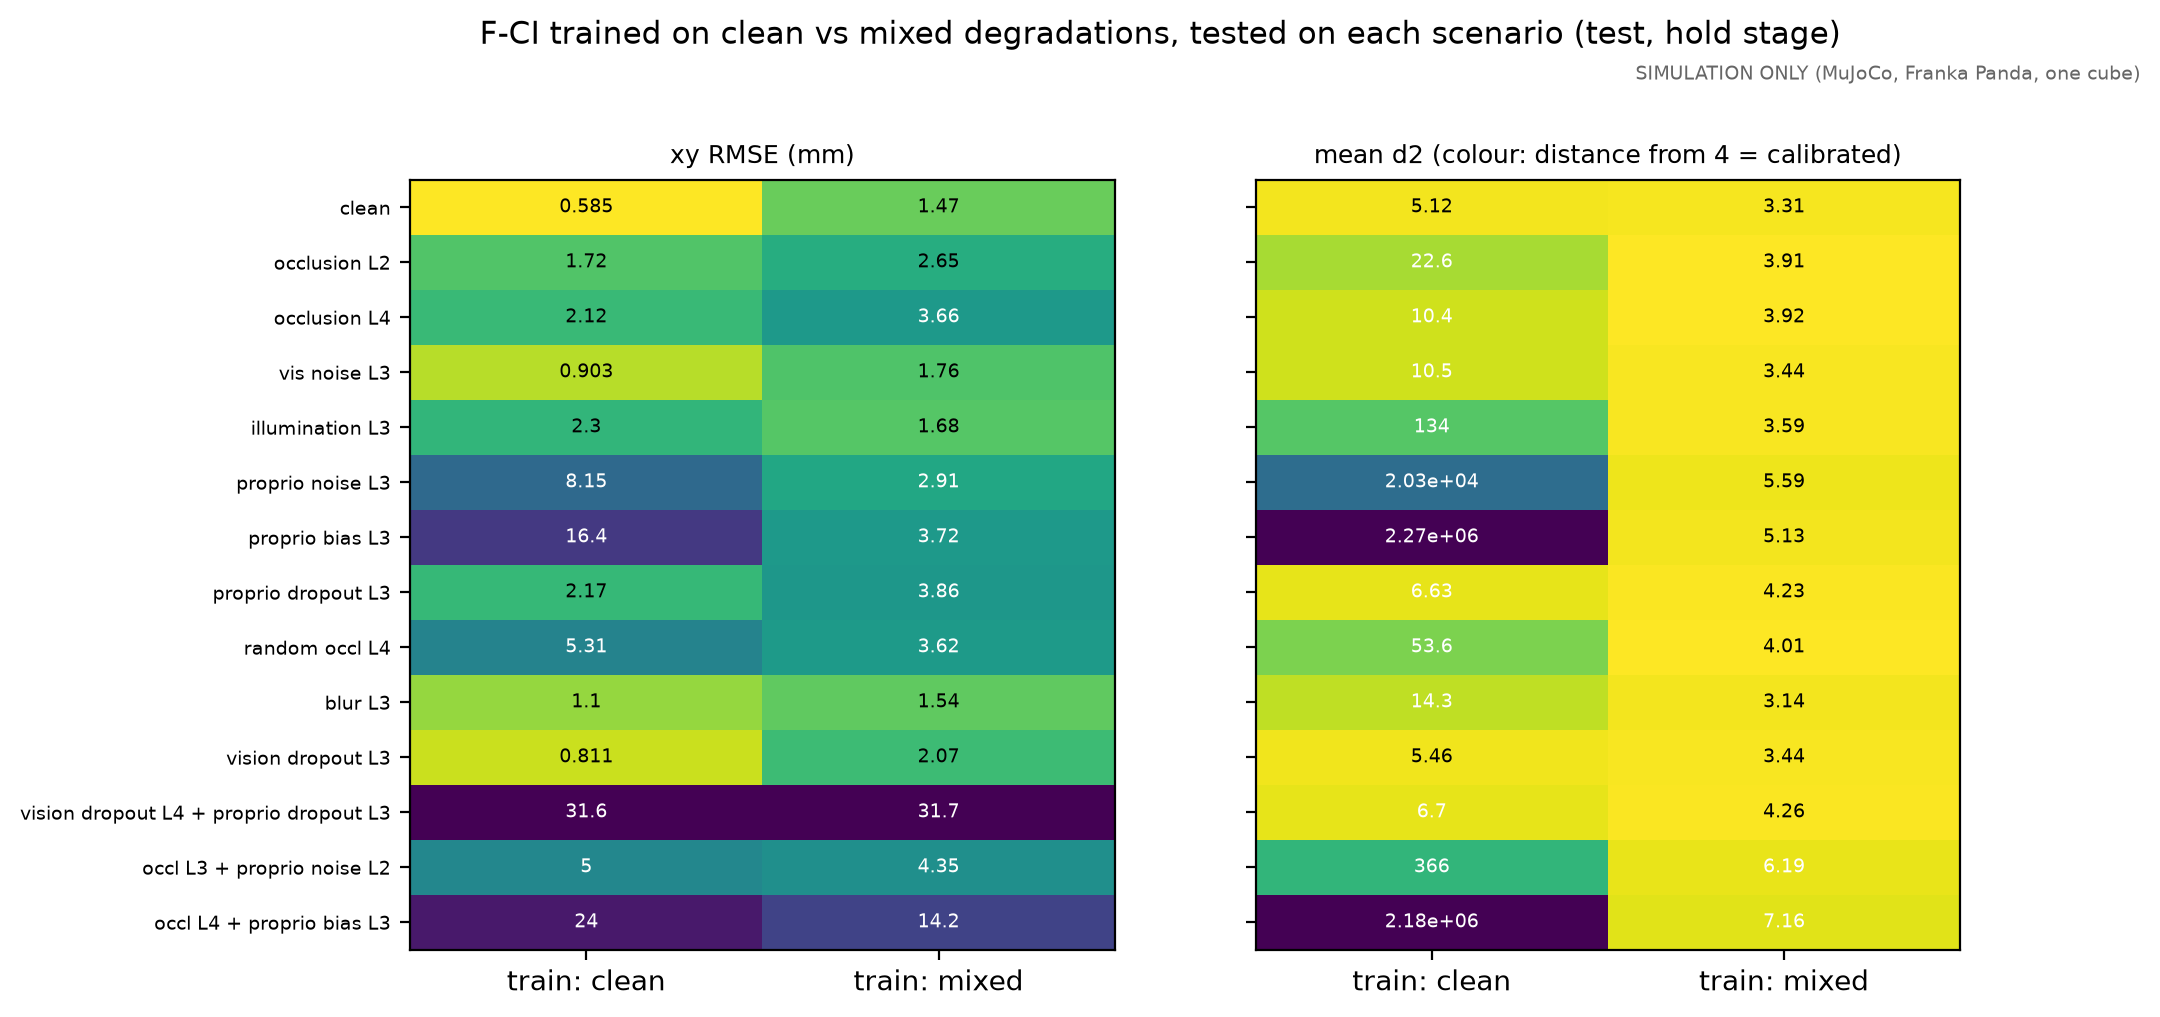
\includegraphics[width=\textwidth]{fig4_clean_vs_mixed_training.png}
\caption{F-CI trained on clean data versus mixed degradations, tested on every scenario. Left: xy RMSE. Right: mean $d^2$, shaded by distance from the calibrated value 4. Simulation only.}
\label{fig:matrix}
\end{figure}

\subsection{Ablation: the contact expert and expert weights}
\begin{figure}[t]
\centering
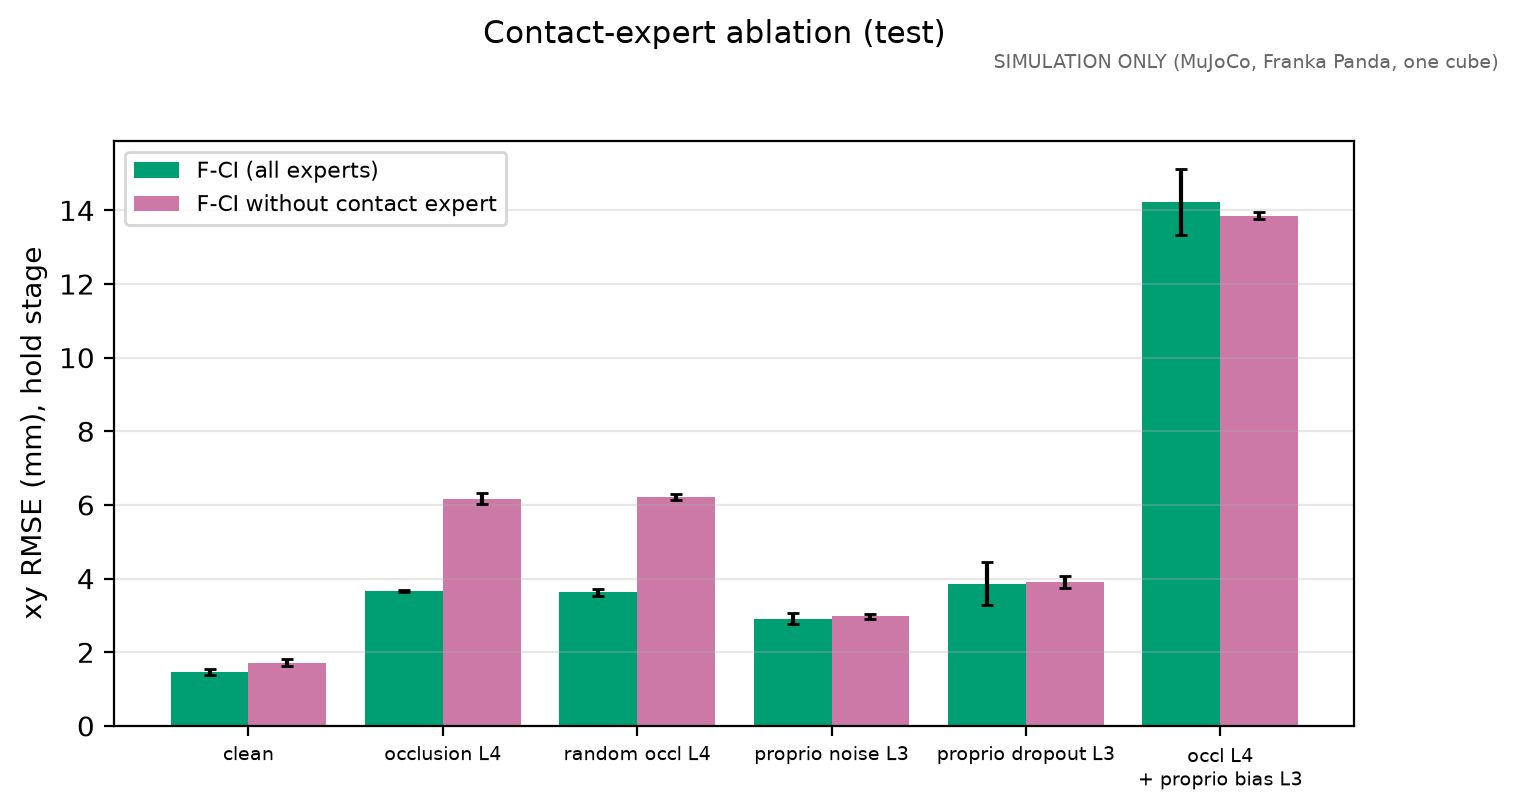
\includegraphics[width=0.78\textwidth]{fig6_contact_ablation.png}
\caption{Removing the contact expert from F-CI (mixed training). Simulation only.}
\label{fig:contact}
\end{figure}
Removing the contact expert raises the error when vision is degraded: occlusion L4 3.7 $\to$ 6.2\,mm ($\Delta=-2.5$\,mm with the expert, CI $[-2.8,-2.3]$), random rectangles 3.6 $\to$ 6.2\,mm, vision dropout 2.1 $\to$ 3.1\,mm, and clean 1.5 $\to$ 1.7\,mm (Fig.~\ref{fig:contact}). It makes no practical difference under proprioceptive noise or dropout (differences $\le0.06$\,mm) and it slightly hurts under strong contact noise (1.9 versus 1.7\,mm). This contradicts the earlier validation-seed impression that the contact expert contributes little; the pre-registration was corrected \emph{before} the test split was used.

The covariance-intersection weights (Fig.~\ref{fig:weights}) behave sensibly: the vision weight is about 0.4 on clean data and drops to roughly 0.03 under occlusion L4 and below 0.01 under random occlusion; trust moves to proprioception and contact. Under proprioceptive faults the vision weight rises to about 0.5--0.6.

\begin{figure}[t]
\centering
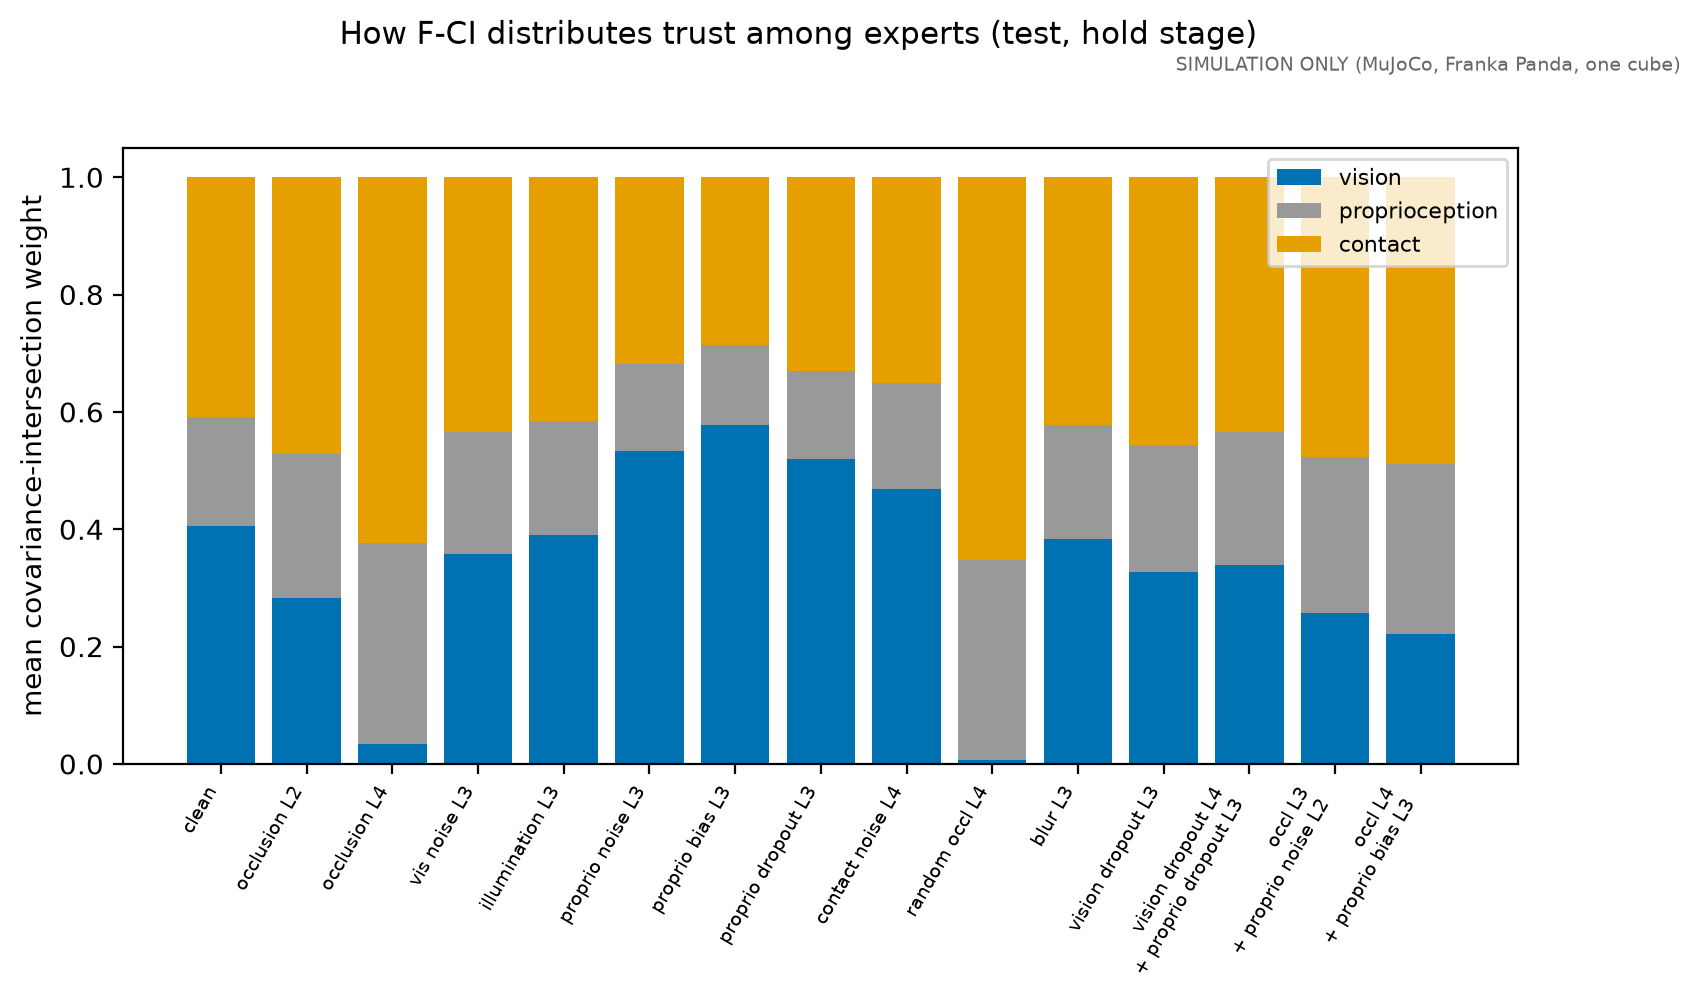
\includegraphics[width=0.9\textwidth]{fig5_expert_weights.png}
\caption{Mean covariance-intersection weights of the three experts per scenario (hold stage). Simulation only.}
\label{fig:weights}
\end{figure}

\subsection{Out-of-distribution cube positions (test\_ood)}
On test\_ood (100 episodes with cube positions outside the training range), vision-only degrades strongly (28.5\,mm on clean data, against 3.5\,mm in distribution) while F-CI degrades less (4.5\,mm). The same pre-registered rules give:
H1 \emph{supported} (gains of 25.8, 40.9 and 113.1\,mm; relative gain 0.86 under occlusion L4 versus 0.84 on clean, contrast CI $[0.00,0.04]$, i.e.\ barely beyond the pre-registered criterion); the stress scenario now \emph{favours} fusion (25.8 versus 47.3\,mm), because vision-only is unreliable out of range;
H2 \emph{supported} but exactly at the threshold (NLL gains in 6 of 9 scenarios for each comparator, none less accurate);
H3 \emph{partially supported} (mixed training again lowers NLL by orders of magnitude; non-inferiority to the control holds in the second combination (RMSE ratio upper bound 1.14, $\Delta$NLL bound $-1.2$) but not in the first (1.11, $+0.66$)). These OOD results should be read as secondary, since test\_ood was not part of the primary decision rules.

%==============================================================================
\section{Discussion}
\paragraph{What the evidence supports.}
A fusion model that treats each modality as a calibrated Gaussian expert and combines them with covariance-intersection weights is the most accurate \emph{and} the best calibrated of the learned fusion approaches in the hold stage, in a simulated setting where the three modalities have genuinely different failure modes. It degrades gracefully when proprioception fails (3.9\,mm against 22--28\,mm for monolithic fusion) or vision fails, and its reported uncertainty is usable (coverage close to nominal, error tracks predicted $\sigma$). Mixed-degradation training is what makes uncertainty trustworthy under failures that were not seen in clean training.

\paragraph{What it does not support.}
(1) The claim that fusion helps \emph{particularly} under occlusion is weak: it helps nearly as much without any degradation. (2) Fusion is not uniformly better than vision-only: a constant proprioceptive bias plus heavy occlusion makes it worse, and over all frames occlusion L4 it is slightly worse. (3) Mixed training does not give full generalisation to unseen combinations, and it costs clean accuracy. (4) These are single-simulation results with three training seeds, one cube and one camera.

\paragraph{Why monolithic fusion fails when a modality drops out.}
F0--F2 were trained on the same data, but their joint embedding must \emph{learn} what to do for every availability pattern; with proprioceptive dropout they produce errors of 22--29\,mm, close to the error of the proprioceptive model alone (50\,mm), i.e.\ they follow the missing modality. The expert/information-form structure makes ``ignore an unavailable expert'' a property of the architecture rather than of the data.

\paragraph{Mismatch to the pre-registered predictions.}
Two of our validation-based expectations were wrong or only weakly right: the contact expert is useful (not marginal), and the relative gain under occlusion is barely larger than on clean data.

%==============================================================================
\section{Threats to validity: leaks found during development}
\label{sec:leaks}
Several issues that would have inflated the results were found by controls and fixed \emph{before} the final protocol. We list them because they show how easily a per-frame, simulated estimator can appear to work for the wrong reason.
\begin{enumerate}
\item \textbf{Policy leakage through proprioception.} The scripted hand hovers above the cube, so joint angles reveal the cube position even though the arm does not touch it. Fix: proprioceptive inputs and the kinematic estimate are gated to the holding phase; results are reported per stage.
\item \textbf{Occluder leakage.} A grey square centred on the cube revealed its position; a control that re-renders episodes with an invisible cube (physics unchanged) still gave 6--11\,mm. Fix: decoy squares around the occluder; random-rectangle occlusion and a vision-dropout family were added. A residual cue from the arm remains outside the hold stage (7--11\,mm on validation).
\item \textbf{Contact-feature leakage.} The TCP $x,y$ in the contact features predicted the cube position outside the grasp ($R^2=0.998$). Fix: removed; a regression test checks it.
\item \textbf{Classical-fusion prior bug.} When proprioception was missing the classical fusion wrongly assumed the cube was on the table; fixed with a broad height prior and a regression test.
\item \textbf{Numerical issues.} A constant input feature with near-zero variance gave standardised values of $-10^{6}$ and a 25\,m error; fixed with a standard-deviation floor and clamping. Loss spikes at the MSE$\to$NLL switch were fixed as described in Section~\ref{sec:nll}.
\end{enumerate}

\paragraph{Remaining limitations.}
Models are \emph{per frame} (no temporal filter), so frames with nothing observable fall back to the prior. There is one cube, one camera and a scripted policy; the cube position is uniformly random in a small workspace. The 4-D Gaussian is a crude model of yaw when yaw is unobservable. Confidence intervals are over episodes of a single simulated environment and three training seeds; with few seeds, standard deviations are themselves uncertain. Bit-exact reproduction of trained models across machines is not guaranteed (GPU non-determinism); data generation and all degradations are deterministic given the seeds. Nothing here says how the methods behave on a real robot.

%==============================================================================
\section{Reproducibility}
All code is in a modular repository with configuration files (no hard-coded paths), checkpointing with atomic writes and resume, JSON-lines logging and a unit-test suite (more than 90 tests, covering the loss, covariance positive-definiteness, degradations, leak regressions, fusion rules and statistics). Data generation uses fixed seeds and episode-level splits; the protocol runner fingerprints all configuration files and the dataset manifest; the pre-registration is frozen by a SHA-256 hash recorded before the test split was evaluated. The tables in this report are generated by a script from the saved evaluation output, not typed by hand. The command sequence is: generate data; \texttt{run\_protocol.py}; \texttt{evaluate\_all.py} on validation, test and test\_ood; \texttt{analyze.py}; \texttt{make\_figures.py}.

\section{Conclusion}
In this \simonly{} study, treating modalities as calibrated Gaussian experts fused with covariance intersection gave the best accuracy and calibration among the compared learned fusion models when sensors degrade, with clear qualifications: a modest ``particularly under occlusion'' effect, a failure case under proprioceptive bias with heavy occlusion, a calibration-dominated (rather than accuracy-dominated) benefit of degradation-aware training, and incomplete generalisation to unseen failure combinations. Closing these gaps (temporal filtering, bias-aware proprioceptive experts, richer scenes, real data) is future work.

\begin{thebibliography}{99}\small
\bibitem{todorov2012mujoco} E.~Todorov, T.~Erez, Y.~Tassa. MuJoCo: A physics engine for model-based control. IROS, 2012.
\bibitem{menagerie} Google DeepMind. MuJoCo Menagerie: a collection of high-quality models for MuJoCo. \url{https://github.com/google-deepmind/mujoco_menagerie}.
\bibitem{kendall2017} A.~Kendall, Y.~Gal. What uncertainties do we need in Bayesian deep learning for computer vision? NeurIPS, 2017.
\bibitem{nix1994} D.~A.~Nix, A.~S.~Weigend. Estimating the mean and variance of the target probability distribution. ICNN, 1994.
\bibitem{seitzer2022} M.~Seitzer, A.~Tavakoli, D.~Antic, G.~Martius. On the pitfalls of heteroscedastic uncertainty estimation with probabilistic neural networks. ICLR, 2022.
\bibitem{lakshminarayanan2017} B.~Lakshminarayanan, A.~Pritzel, C.~Blundell. Simple and scalable predictive uncertainty estimation using deep ensembles. NeurIPS, 2017.
\bibitem{guo2017} C.~Guo, G.~Pleiss, Y.~Sun, K.~Q.~Weinberger. On calibration of modern neural networks. ICML, 2017.
\bibitem{julier1997non} S.~Julier, J.~Uhlmann. A non-divergent estimation algorithm in the presence of unknown correlations. American Control Conference, 1997.
\bibitem{hinton2002} G.~E.~Hinton. Training products of experts by minimizing contrastive divergence. Neural Computation, 14(8), 2002.
\bibitem{finn2016deep} C.~Finn, X.~Y.~Tan, Y.~Duan, T.~Darrell, S.~Levine, P.~Abbeel. Deep spatial autoencoders for visuomotor learning. ICRA, 2016.
\bibitem{lee2019} M.~A.~Lee, Y.~Zhu, K.~Srinivasan, P.~Shah, S.~Savarese, L.~Fei-Fei, A.~Garg, J.~Bohg. Making sense of vision and touch: self-supervised learning of multimodal representations for contact-rich tasks. ICRA, 2019.
\bibitem{holm1979} S.~Holm. A simple sequentially rejective multiple test procedure. Scandinavian Journal of Statistics, 6(2), 1979.
\bibitem{efron1979} B.~Efron. Bootstrap methods: another look at the jackknife. Annals of Statistics, 7(1), 1979.
\end{thebibliography}

\clearpage
\appendix
\section{Complete test-split tables}
\label{app:tables}
All tables: test split, hold (\texttt{coupled}) stage, mean$\pm$std over 3 training seeds, \simonly{}. Models: Vis = vision-only, Prop = gated proprioception, F0--F2 = non-uncertainty-aware fusion, PoE/tPoE/F-CI = uncertainty-aware fusion with the respective rule, F-CI$_{\mathrm{clean}}$ = F-CI trained on clean data only, WLS = classical WLS fusion with oracle noise levels.
\begin{table*}[p]\centering\scriptsize\setlength{\tabcolsep}{3pt}
\resizebox{\textwidth}{!}{%
\begin{tabular}{lrrrrrrrrrr}\toprule
Scenario & Vis & Prop & F0 & F1 & F2 & PoE & tPoE & F-CI & F-CI$_{\mathrm{clean}}$ & WLS \\\midrule
clean & $3.5{\pm}0.2$ & $7.1{\pm}0.2$ & $2.1{\pm}0.6$ & $3.0{\pm}1.2$ & $3.9{\pm}2.4$ & $1.4{\pm}0.0$ & $1.4{\pm}0.2$ & $1.5{\pm}0.1$ & $0.6{\pm}0.0$ & $5.1$ \\
occlusion L2 & $4.9{\pm}0.3$ & $7.1{\pm}0.2$ & $3.0{\pm}0.3$ & $4.9{\pm}1.7$ & $5.5{\pm}2.6$ & $2.4{\pm}0.1$ & $2.4{\pm}0.2$ & $2.6{\pm}0.3$ & $1.7{\pm}0.1$ & $5.9$ \\
occlusion L4 & $10.3{\pm}0.7$ & $7.1{\pm}0.2$ & $5.8{\pm}0.5$ & $5.9{\pm}1.2$ & $6.8{\pm}2.7$ & $3.8{\pm}0.1$ & $3.7{\pm}0.1$ & $3.7{\pm}0.0$ & $2.1{\pm}0.3$ & $5.2$ \\
vis noise L3 & $4.0{\pm}0.2$ & $7.1{\pm}0.2$ & $2.3{\pm}0.5$ & $3.3{\pm}1.2$ & $4.1{\pm}2.3$ & $1.7{\pm}0.1$ & $1.7{\pm}0.2$ & $1.8{\pm}0.1$ & $0.9{\pm}0.1$ & $5.2$ \\
illumination L3 & $4.5{\pm}0.2$ & $7.1{\pm}0.2$ & $2.2{\pm}0.6$ & $3.2{\pm}1.2$ & $4.1{\pm}2.2$ & $1.6{\pm}0.0$ & $1.6{\pm}0.2$ & $1.7{\pm}0.1$ & $2.3{\pm}0.4$ & $5.1$ \\
proprio noise L3 & $3.5{\pm}0.2$ & $12.0{\pm}0.2$ & $3.3{\pm}0.7$ & $4.4{\pm}1.1$ & $5.4{\pm}2.4$ & $2.9{\pm}0.0$ & $2.9{\pm}0.2$ & $2.9{\pm}0.2$ & $8.2{\pm}0.2$ & $12.0$ \\
proprio bias L3 & $3.5{\pm}0.2$ & $31.4{\pm}0.1$ & $7.3{\pm}0.6$ & $10.7{\pm}2.7$ & $11.9{\pm}2.7$ & $3.9{\pm}0.1$ & $3.7{\pm}0.2$ & $3.7{\pm}0.2$ & $16.4{\pm}0.6$ & $35.9$ \\
proprio dropout L3 & $3.5{\pm}0.2$ & $50.0{\pm}0.0$ & $29.2{\pm}3.1$ & $22.2{\pm}6.7$ & $28.3{\pm}1.8$ & $3.9{\pm}0.4$ & $3.4{\pm}0.2$ & $3.9{\pm}0.6$ & $2.2{\pm}0.6$ & $30.7$ \\
contact noise L2 & $3.5{\pm}0.2$ & $7.1{\pm}0.2$ & $2.3{\pm}0.6$ & $3.3{\pm}1.2$ & $4.2{\pm}2.3$ & $1.5{\pm}0.0$ & $1.5{\pm}0.2$ & $1.6{\pm}0.1$ & $6.0{\pm}0.1$ & $5.6$ \\
contact noise L4 & $3.5{\pm}0.2$ & $7.1{\pm}0.2$ & $2.8{\pm}0.6$ & $3.8{\pm}1.3$ & $5.0{\pm}2.8$ & $1.7{\pm}0.0$ & $1.8{\pm}0.2$ & $1.9{\pm}0.1$ & $16.3{\pm}0.8$ & $5.7$ \\
random occl L4 & $48.4{\pm}0.1$ & $7.1{\pm}0.2$ & $5.8{\pm}0.9$ & $6.2{\pm}1.2$ & $7.4{\pm}2.9$ & $3.7{\pm}0.1$ & $3.6{\pm}0.1$ & $3.6{\pm}0.1$ & $5.3{\pm}1.8$ & $5.2$ \\
blur L3 & $3.4{\pm}0.1$ & $7.1{\pm}0.2$ & $2.2{\pm}0.6$ & $3.1{\pm}1.1$ & $3.9{\pm}2.3$ & $1.5{\pm}0.0$ & $1.4{\pm}0.2$ & $1.5{\pm}0.1$ & $1.1{\pm}0.1$ & $4.8$ \\
vision dropout L3 & $50.5{\pm}0.2$ & $7.1{\pm}0.2$ & $3.2{\pm}0.6$ & $4.0{\pm}1.3$ & $4.9{\pm}2.5$ & $2.0{\pm}0.0$ & $2.0{\pm}0.1$ & $2.1{\pm}0.1$ & $0.8{\pm}0.0$ & $5.2$ \\
vision dropout L4 {+} proprio dropout L3 & $72.9{\pm}0.2$ & $50.0{\pm}0.0$ & $39.2{\pm}1.0$ & $36.3{\pm}2.6$ & $38.6{\pm}1.2$ & $31.8{\pm}0.0$ & $31.7{\pm}0.0$ & $31.7{\pm}0.0$ & $31.6{\pm}0.0$ & $40.3$ \\
occl L3 {+} proprio noise L2 & $6.3{\pm}0.6$ & $8.0{\pm}0.2$ & $4.2{\pm}0.4$ & $6.0{\pm}1.5$ & $6.8{\pm}2.6$ & $4.2{\pm}0.2$ & $4.2{\pm}0.2$ & $4.3{\pm}0.4$ & $5.0{\pm}0.1$ & $7.8$ \\
occl L4 {+} proprio bias L3 & $10.3{\pm}0.7$ & $31.4{\pm}0.1$ & $17.6{\pm}0.6$ & $14.7{\pm}0.9$ & $16.2{\pm}2.9$ & $12.1{\pm}1.1$ & $12.1{\pm}0.7$ & $14.2{\pm}0.9$ & $24.0{\pm}2.7$ & $34.7$ \\
\bottomrule\end{tabular}}
\caption{Test split, hold (\texttt{coupled}) stage: xy RMSE in mm, mean$\pm$std over 3 training seeds (WLS: classical fusion given the true noise levels, one deterministic run). Vis/Prop: vision-only / gated-proprioception models trained on mixed degradations; F0--F2: non-uncertainty-aware fusion; F-CI$_{\mathrm{clean}}$ trained on clean data only; all others trained on mixed degradations.}\label{tab:app_rmse}\end{table*}

\begin{table*}[p]\centering\scriptsize\setlength{\tabcolsep}{3pt}
\resizebox{\textwidth}{!}{%
\begin{tabular}{lrrrrrrrrrr}\toprule
Scenario & Vis & Prop & F0 & F1 & F2 & PoE & tPoE & F-CI & F-CI$_{\mathrm{clean}}$ & WLS \\\midrule
clean & $5.7{\pm}0.1$ & $8.9{\pm}3.6$ & $4.3{\pm}0.2$ & $4.0{\pm}0.7$ & $3.5{\pm}0.3$ & $7.2{\pm}0.5$ & $5.3{\pm}0.0$ & $3.3{\pm}0.2$ & $5.1{\pm}0.4$ & $3.7$ \\
occlusion L2 & $8.5{\pm}0.9$ & $8.9{\pm}3.6$ & $6.0{\pm}0.7$ & $6.2{\pm}0.9$ & $4.8{\pm}0.2$ & $20.2{\pm}15.8$ & $5.8{\pm}0.1$ & $3.9{\pm}0.5$ & $22.6{\pm}5.9$ & $5.9$ \\
occlusion L4 & $131.8{\pm}96.8$ & $8.9{\pm}3.6$ & $4.9{\pm}0.4$ & $5.3{\pm}1.3$ & $4.3{\pm}0.5$ & $7.3{\pm}0.7$ & $5.0{\pm}0.2$ & $3.9{\pm}0.1$ & $10.4{\pm}2.7$ & $2.9$ \\
vis noise L3 & $6.0{\pm}0.2$ & $8.9{\pm}3.6$ & $4.7{\pm}0.2$ & $4.4{\pm}0.4$ & $3.9{\pm}0.3$ & $7.7{\pm}0.6$ & $5.6{\pm}0.2$ & $3.4{\pm}0.1$ & $10.5{\pm}2.1$ & $4.0$ \\
illumination L3 & $7.4{\pm}0.5$ & $8.9{\pm}3.6$ & $4.5{\pm}0.1$ & $4.3{\pm}0.6$ & $3.8{\pm}0.3$ & $10.0{\pm}1.2$ & $5.6{\pm}0.2$ & $3.6{\pm}0.2$ & $133.6{\pm}158.1$ & $3.7$ \\
proprio noise L3 & $5.7{\pm}0.1$ & $6.7{\pm}0.4$ & $7.2{\pm}0.5$ & $6.5{\pm}0.5$ & $6.0{\pm}0.7$ & $11.9{\pm}0.7$ & $7.6{\pm}0.2$ & $5.6{\pm}0.2$ & $2.0\!\times\!10^{4}{\pm}5.5\!\times\!10^{3}$ & $6.8$ \\
proprio bias L3 & $5.7{\pm}0.1$ & $11.2{\pm}2.6$ & $8.6{\pm}0.6$ & $9.3{\pm}1.2$ & $8.5{\pm}0.8$ & $9.6{\pm}0.5$ & $5.8{\pm}0.3$ & $5.1{\pm}0.4$ & $2.3\!\times\!10^{6}{\pm}1.0\!\times\!10^{6}$ & $585.5$ \\
proprio dropout L3 & $5.7{\pm}0.1$ & $11.6{\pm}2.9$ & $8.2{\pm}0.4$ & $5.0{\pm}0.5$ & $5.3{\pm}1.0$ & $7.1{\pm}0.7$ & $5.7{\pm}0.1$ & $4.2{\pm}0.4$ & $6.6{\pm}0.6$ & $4.4$ \\
contact noise L2 & $5.7{\pm}0.1$ & $8.9{\pm}3.6$ & $4.7{\pm}0.3$ & $4.4{\pm}0.6$ & $3.9{\pm}0.4$ & $7.6{\pm}0.5$ & $5.5{\pm}0.1$ & $3.5{\pm}0.3$ & $420.6{\pm}32.3$ & $4.1$ \\
contact noise L4 & $5.7{\pm}0.1$ & $8.9{\pm}3.6$ & $5.5{\pm}0.2$ & $5.1{\pm}0.5$ & $4.7{\pm}0.5$ & $7.7{\pm}0.4$ & $5.3{\pm}0.1$ & $3.7{\pm}0.3$ & $1.6\!\times\!10^{4}{\pm}7.3\!\times\!10^{3}$ & $4.1$ \\
random occl L4 & $6.1{\pm}1.4$ & $8.9{\pm}3.6$ & $4.0{\pm}0.3$ & $4.4{\pm}1.3$ & $4.0{\pm}0.7$ & $7.4{\pm}0.9$ & $5.0{\pm}0.2$ & $4.0{\pm}0.1$ & $53.6{\pm}42.9$ & $2.9$ \\
blur L3 & $5.5{\pm}0.5$ & $8.9{\pm}3.6$ & $4.5{\pm}0.3$ & $4.1{\pm}0.5$ & $3.6{\pm}0.3$ & $6.8{\pm}0.3$ & $5.2{\pm}0.0$ & $3.1{\pm}0.1$ & $14.3{\pm}1.5$ & $3.3$ \\
vision dropout L3 & $5.7{\pm}0.1$ & $8.9{\pm}3.6$ & $4.2{\pm}0.2$ & $4.1{\pm}0.7$ & $3.6{\pm}0.3$ & $7.2{\pm}0.5$ & $5.4{\pm}0.1$ & $3.4{\pm}0.2$ & $5.5{\pm}0.3$ & $3.6$ \\
vision dropout L4 {+} proprio dropout L3 & $5.9{\pm}0.1$ & $11.6{\pm}2.9$ & $6.7{\pm}0.2$ & $4.9{\pm}0.5$ & $4.9{\pm}0.8$ & $7.0{\pm}0.6$ & $5.8{\pm}0.1$ & $4.3{\pm}0.2$ & $6.7{\pm}0.3$ & $4.0$ \\
occl L3 {+} proprio noise L2 & $7.5{\pm}0.6$ & $8.0{\pm}2.0$ & $7.0{\pm}0.4$ & $6.9{\pm}1.1$ & $5.7{\pm}0.1$ & $13.7{\pm}1.2$ & $8.4{\pm}0.2$ & $6.2{\pm}0.4$ & $366.0{\pm}33.6$ & $6.7$ \\
occl L4 {+} proprio bias L3 & $131.8{\pm}96.8$ & $11.2{\pm}2.6$ & $12.5{\pm}1.5$ & $13.9{\pm}1.9$ & $11.5{\pm}0.7$ & $14.7{\pm}2.1$ & $8.2{\pm}0.2$ & $7.2{\pm}0.1$ & $2.2\!\times\!10^{6}{\pm}8.3\!\times\!10^{5}$ & $585.5$ \\
\bottomrule\end{tabular}}
\caption{Test split, hold stage: mean squared Mahalanobis distance $d^2$ (calibrated $=4$ for a 4-D Gaussian; values $\ge 10^3$ in scientific notation). Same models as Table~\ref{tab:app_rmse}.}\label{tab:app_d2}\end{table*}

\begin{table*}[p]\centering\scriptsize\setlength{\tabcolsep}{3pt}
\resizebox{\textwidth}{!}{%
\begin{tabular}{lrrrrrrrrrr}\toprule
Scenario & Vis & Prop & F0 & F1 & F2 & PoE & tPoE & F-CI & F-CI$_{\mathrm{clean}}$ & WLS \\\midrule
clean & $0.86{\pm}0.00$ & $0.73{\pm}0.12$ & $0.91{\pm}0.01$ & $0.93{\pm}0.03$ & $0.95{\pm}0.02$ & $0.77{\pm}0.01$ & $0.87{\pm}0.00$ & $0.96{\pm}0.01$ & $0.87{\pm}0.01$ & $0.95$ \\
occlusion L2 & $0.77{\pm}0.01$ & $0.73{\pm}0.12$ & $0.83{\pm}0.03$ & $0.81{\pm}0.06$ & $0.89{\pm}0.01$ & $0.71{\pm}0.02$ & $0.84{\pm}0.01$ & $0.94{\pm}0.02$ & $0.55{\pm}0.05$ & $0.83$ \\
occlusion L4 & $0.89{\pm}0.02$ & $0.73{\pm}0.12$ & $0.89{\pm}0.03$ & $0.86{\pm}0.07$ & $0.92{\pm}0.03$ & $0.75{\pm}0.03$ & $0.88{\pm}0.01$ & $0.94{\pm}0.01$ & $0.70{\pm}0.08$ & $1.00$ \\
vis noise L3 & $0.85{\pm}0.00$ & $0.73{\pm}0.12$ & $0.90{\pm}0.02$ & $0.91{\pm}0.02$ & $0.94{\pm}0.02$ & $0.75{\pm}0.02$ & $0.85{\pm}0.01$ & $0.96{\pm}0.01$ & $0.63{\pm}0.07$ & $0.94$ \\
illumination L3 & $0.84{\pm}0.00$ & $0.73{\pm}0.12$ & $0.90{\pm}0.01$ & $0.92{\pm}0.03$ & $0.94{\pm}0.02$ & $0.74{\pm}0.03$ & $0.86{\pm}0.01$ & $0.96{\pm}0.01$ & $0.57{\pm}0.02$ & $0.95$ \\
proprio noise L3 & $0.86{\pm}0.00$ & $0.80{\pm}0.01$ & $0.75{\pm}0.03$ & $0.80{\pm}0.03$ & $0.83{\pm}0.04$ & $0.62{\pm}0.00$ & $0.76{\pm}0.01$ & $0.86{\pm}0.01$ & $0.01{\pm}0.00$ & $0.83$ \\
proprio bias L3 & $0.86{\pm}0.00$ & $0.67{\pm}0.02$ & $0.68{\pm}0.03$ & $0.66{\pm}0.06$ & $0.68{\pm}0.03$ & $0.73{\pm}0.01$ & $0.85{\pm}0.02$ & $0.89{\pm}0.01$ & $0.04{\pm}0.01$ & $0.03$ \\
proprio dropout L3 & $0.86{\pm}0.00$ & $0.64{\pm}0.10$ & $0.84{\pm}0.01$ & $0.89{\pm}0.02$ & $0.90{\pm}0.01$ & $0.79{\pm}0.01$ & $0.86{\pm}0.00$ & $0.93{\pm}0.01$ & $0.82{\pm}0.02$ & $0.92$ \\
contact noise L2 & $0.86{\pm}0.00$ & $0.73{\pm}0.12$ & $0.90{\pm}0.02$ & $0.92{\pm}0.03$ & $0.94{\pm}0.02$ & $0.75{\pm}0.01$ & $0.86{\pm}0.01$ & $0.96{\pm}0.01$ & $0.11{\pm}0.01$ & $0.94$ \\
contact noise L4 & $0.86{\pm}0.00$ & $0.73{\pm}0.12$ & $0.86{\pm}0.01$ & $0.88{\pm}0.02$ & $0.90{\pm}0.03$ & $0.76{\pm}0.01$ & $0.87{\pm}0.01$ & $0.95{\pm}0.02$ & $0.03{\pm}0.01$ & $0.94$ \\
random occl L4 & $0.94{\pm}0.01$ & $0.73{\pm}0.12$ & $0.94{\pm}0.01$ & $0.90{\pm}0.07$ & $0.93{\pm}0.04$ & $0.78{\pm}0.02$ & $0.88{\pm}0.02$ & $0.94{\pm}0.01$ & $0.68{\pm}0.06$ & $1.00$ \\
blur L3 & $0.89{\pm}0.02$ & $0.73{\pm}0.12$ & $0.91{\pm}0.01$ & $0.93{\pm}0.02$ & $0.95{\pm}0.02$ & $0.79{\pm}0.02$ & $0.87{\pm}0.00$ & $0.98{\pm}0.01$ & $0.51{\pm}0.04$ & $0.97$ \\
vision dropout L3 & $0.87{\pm}0.00$ & $0.73{\pm}0.12$ & $0.91{\pm}0.01$ & $0.93{\pm}0.03$ & $0.95{\pm}0.01$ & $0.77{\pm}0.02$ & $0.86{\pm}0.00$ & $0.96{\pm}0.01$ & $0.86{\pm}0.01$ & $0.96$ \\
vision dropout L4 {+} proprio dropout L3 & $0.88{\pm}0.00$ & $0.64{\pm}0.10$ & $0.84{\pm}0.00$ & $0.88{\pm}0.02$ & $0.91{\pm}0.02$ & $0.80{\pm}0.01$ & $0.86{\pm}0.00$ & $0.94{\pm}0.01$ & $0.82{\pm}0.01$ & $0.95$ \\
occl L3 {+} proprio noise L2 & $0.79{\pm}0.01$ & $0.74{\pm}0.07$ & $0.77{\pm}0.02$ & $0.77{\pm}0.06$ & $0.85{\pm}0.00$ & $0.52{\pm}0.02$ & $0.69{\pm}0.01$ & $0.82{\pm}0.02$ & $0.01{\pm}0.00$ & $0.83$ \\
occl L4 {+} proprio bias L3 & $0.89{\pm}0.02$ & $0.67{\pm}0.02$ & $0.55{\pm}0.05$ & $0.49{\pm}0.07$ & $0.56{\pm}0.02$ & $0.61{\pm}0.02$ & $0.77{\pm}0.00$ & $0.82{\pm}0.01$ & $0.00{\pm}0.00$ & $0.03$ \\
\bottomrule\end{tabular}}
\caption{Test split, hold stage: empirical coverage of the nominal 95\,\% ellipsoid (calibrated $=0.95$).}\label{tab:app_cov}\end{table*}

\begin{table*}[p]\centering\scriptsize\setlength{\tabcolsep}{3pt}
\resizebox{\textwidth}{!}{%
\begin{tabular}{lrrrrrrrrrr}\toprule
Scenario & Vis & Prop & F0 & F1 & F2 & PoE & tPoE & F-CI & F-CI$_{\mathrm{clean}}$ & WLS \\\midrule
clean & $-15.7{\pm}0.1$ & $-13.0{\pm}1.2$ & $-17.1{\pm}1.0$ & $-15.7{\pm}1.5$ & $-15.5{\pm}1.8$ & $-18.0{\pm}0.2$ & $-18.5{\pm}0.5$ & $-18.4{\pm}0.1$ & $-20.6{\pm}0.1$ & $-14.8$ \\
occlusion L2 & $-12.6{\pm}0.3$ & $-13.0{\pm}1.2$ & $-15.4{\pm}0.4$ & $-13.8{\pm}1.3$ & $-14.0{\pm}1.3$ & $-10.4{\pm}7.9$ & $-16.9{\pm}0.2$ & $-17.0{\pm}0.2$ & $-11.5{\pm}2.9$ & $-13.5$ \\
occlusion L4 & $53.9{\pm}48.4$ & $-13.0{\pm}1.2$ & $-13.8{\pm}0.3$ & $-13.4{\pm}0.9$ & $-13.4{\pm}1.2$ & $-15.9{\pm}0.4$ & $-16.4{\pm}0.0$ & $-16.5{\pm}0.1$ & $-17.4{\pm}1.3$ & $-14.7$ \\
vis noise L3 & $-14.7{\pm}0.1$ & $-13.0{\pm}1.2$ & $-16.5{\pm}0.8$ & $-15.4{\pm}1.4$ & $-15.2{\pm}1.6$ & $-17.3{\pm}0.2$ & $-17.8{\pm}0.3$ & $-17.8{\pm}0.1$ & $-17.9{\pm}1.0$ & $-14.7$ \\
illumination L3 & $-14.5{\pm}0.2$ & $-13.0{\pm}1.2$ & $-16.9{\pm}1.0$ & $-15.5{\pm}1.5$ & $-15.3{\pm}1.7$ & $-16.4{\pm}0.6$ & $-18.1{\pm}0.5$ & $-18.1{\pm}0.1$ & $43.9{\pm}79.0$ & $-14.8$ \\
proprio noise L3 & $-15.7{\pm}0.1$ & $-11.1{\pm}0.3$ & $-15.3{\pm}0.7$ & $-14.3{\pm}1.2$ & $-14.0{\pm}1.4$ & $-14.2{\pm}0.3$ & $-15.8{\pm}0.6$ & $-16.0{\pm}0.4$ & $1.0\!\times\!10^{4}{\pm}2.8\!\times\!10^{3}$ & $-10.5$ \\
proprio bias L3 & $-15.7{\pm}0.1$ & $-8.4{\pm}1.1$ & $-14.2{\pm}0.7$ & $-12.3{\pm}1.6$ & $-12.4{\pm}1.5$ & $-14.9{\pm}0.2$ & $-16.1{\pm}0.7$ & $-15.9{\pm}0.3$ & $1.1\!\times\!10^{6}{\pm}5.1\!\times\!10^{5}$ & $276.5$ \\
proprio dropout L3 & $-15.7{\pm}0.1$ & $-9.3{\pm}0.9$ & $-13.9{\pm}1.3$ & $-13.7{\pm}1.5$ & $-13.2{\pm}2.2$ & $-17.3{\pm}0.2$ & $-17.7{\pm}0.5$ & $-17.5{\pm}0.2$ & $-19.3{\pm}0.2$ & $-13.1$ \\
contact noise L2 & $-15.7{\pm}0.1$ & $-13.0{\pm}1.2$ & $-16.8{\pm}1.0$ & $-15.5{\pm}1.4$ & $-15.2{\pm}1.7$ & $-17.7{\pm}0.1$ & $-18.3{\pm}0.5$ & $-18.2{\pm}0.1$ & $187.3{\pm}16.1$ & $-14.3$ \\
contact noise L4 & $-15.7{\pm}0.1$ & $-13.0{\pm}1.2$ & $-16.0{\pm}0.9$ & $-14.9{\pm}1.3$ & $-14.6{\pm}1.8$ & $-17.3{\pm}0.1$ & $-17.9{\pm}0.6$ & $-17.7{\pm}0.2$ & $8.2\!\times\!10^{3}{\pm}3.7\!\times\!10^{3}$ & $-14.3$ \\
random occl L4 & $-3.7{\pm}0.6$ & $-13.0{\pm}1.2$ & $-13.9{\pm}0.4$ & $-13.3{\pm}0.9$ & $-13.2{\pm}1.1$ & $-15.8{\pm}0.5$ & $-16.5{\pm}0.0$ & $-16.6{\pm}0.1$ & $4.3{\pm}21.4$ & $-14.7$ \\
blur L3 & $-15.5{\pm}0.3$ & $-13.0{\pm}1.2$ & $-16.8{\pm}0.9$ & $-15.6{\pm}1.4$ & $-15.4{\pm}1.8$ & $-17.9{\pm}0.1$ & $-18.3{\pm}0.4$ & $-18.2{\pm}0.1$ & $-15.9{\pm}0.7$ & $-14.9$ \\
vision dropout L3 & $-12.8{\pm}0.0$ & $-13.0{\pm}1.2$ & $-16.4{\pm}0.9$ & $-15.2{\pm}1.4$ & $-14.9{\pm}1.7$ & $-17.6{\pm}0.2$ & $-18.1{\pm}0.4$ & $-18.0{\pm}0.1$ & $-20.4{\pm}0.1$ & $-14.8$ \\
vision dropout L4 {+} proprio dropout L3 & $-9.8{\pm}0.0$ & $-9.3{\pm}0.9$ & $-12.9{\pm}0.8$ & $-12.5{\pm}1.1$ & $-12.2{\pm}1.7$ & $-15.6{\pm}0.2$ & $-16.0{\pm}0.3$ & $-16.0{\pm}0.1$ & $-17.9{\pm}0.1$ & $-12.6$ \\
occl L3 {+} proprio noise L2 & $-11.9{\pm}0.2$ & $-12.3{\pm}0.6$ & $-14.1{\pm}0.3$ & $-13.0{\pm}1.0$ & $-13.1{\pm}1.1$ & $-12.2{\pm}0.7$ & $-14.0{\pm}0.1$ & $-14.4{\pm}0.3$ & $160.4{\pm}16.8$ & $-10.9$ \\
occl L4 {+} proprio bias L3 & $53.9{\pm}48.4$ & $-8.4{\pm}1.1$ & $-8.9{\pm}0.7$ & $-8.3{\pm}1.1$ & $-9.1{\pm}0.5$ & $-8.1{\pm}1.0$ & $-10.4{\pm}0.2$ & $-10.3{\pm}0.1$ & $1.1\!\times\!10^{6}{\pm}4.2\!\times\!10^{5}$ & $277.2$ \\
\bottomrule\end{tabular}}
\caption{Test split, hold stage: heteroscedastic Gaussian NLL (lower is better; includes the constant, 4-D state).}\label{tab:app_nll}\end{table*}

\begin{table*}[p]\centering\scriptsize\setlength{\tabcolsep}{3pt}
\resizebox{\textwidth}{!}{%
\begin{tabular}{lrrrrrrrrrr}\toprule
Scenario & Vis & Prop & F0 & F1 & F2 & PoE & tPoE & F-CI & F-CI$_{\mathrm{clean}}$ & WLS \\\midrule
clean & $2.4{\pm}0.2$ & $2.8{\pm}0.1$ & $2.1{\pm}0.3$ & $2.6{\pm}0.1$ & $2.6{\pm}0.1$ & $1.7{\pm}0.0$ & $1.7{\pm}0.2$ & $1.8{\pm}0.3$ & $1.1{\pm}0.0$ & $2.7$ \\
occlusion L2 & $3.0{\pm}0.1$ & $2.8{\pm}0.1$ & $2.5{\pm}0.1$ & $2.6{\pm}0.1$ & $2.6{\pm}0.1$ & $2.1{\pm}0.1$ & $2.2{\pm}0.1$ & $2.2{\pm}0.2$ & $4.0{\pm}0.5$ & $2.7$ \\
occlusion L4 & $4.0{\pm}0.1$ & $2.8{\pm}0.1$ & $2.7{\pm}0.1$ & $2.6{\pm}0.1$ & $2.6{\pm}0.2$ & $2.4{\pm}0.0$ & $2.5{\pm}0.0$ & $2.5{\pm}0.0$ & $3.5{\pm}0.6$ & $2.6$ \\
vis noise L3 & $2.6{\pm}0.2$ & $2.8{\pm}0.1$ & $2.3{\pm}0.2$ & $2.6{\pm}0.1$ & $2.6{\pm}0.1$ & $1.8{\pm}0.0$ & $1.9{\pm}0.1$ & $2.0{\pm}0.2$ & $1.8{\pm}0.2$ & $2.7$ \\
illumination L3 & $2.5{\pm}0.2$ & $2.8{\pm}0.1$ & $2.1{\pm}0.2$ & $2.6{\pm}0.1$ & $2.6{\pm}0.1$ & $1.8{\pm}0.0$ & $1.8{\pm}0.2$ & $1.9{\pm}0.3$ & $3.4{\pm}0.2$ & $2.7$ \\
proprio noise L3 & $2.4{\pm}0.2$ & $3.0{\pm}0.1$ & $2.2{\pm}0.3$ & $2.7{\pm}0.1$ & $2.7{\pm}0.1$ & $1.8{\pm}0.0$ & $1.8{\pm}0.2$ & $2.0{\pm}0.3$ & $2.6{\pm}0.1$ & $2.8$ \\
proprio bias L3 & $2.4{\pm}0.2$ & $4.4{\pm}0.1$ & $2.7{\pm}0.5$ & $3.5{\pm}0.3$ & $3.5{\pm}0.4$ & $1.9{\pm}0.1$ & $1.9{\pm}0.3$ & $2.0{\pm}0.3$ & $4.3{\pm}0.3$ & $3.9$ \\
proprio dropout L3 & $2.4{\pm}0.2$ & $7.1{\pm}0.1$ & $2.9{\pm}1.0$ & $4.3{\pm}0.7$ & $4.1{\pm}0.6$ & $1.8{\pm}0.0$ & $1.8{\pm}0.2$ & $1.9{\pm}0.3$ & $1.2{\pm}0.0$ & $5.7$ \\
contact noise L2 & $2.4{\pm}0.2$ & $2.8{\pm}0.1$ & $2.1{\pm}0.3$ & $2.6{\pm}0.1$ & $2.6{\pm}0.1$ & $1.7{\pm}0.0$ & $1.7{\pm}0.2$ & $1.8{\pm}0.3$ & $1.7{\pm}0.0$ & $2.7$ \\
contact noise L4 & $2.4{\pm}0.2$ & $2.8{\pm}0.1$ & $2.2{\pm}0.3$ & $2.6{\pm}0.1$ & $2.7{\pm}0.2$ & $1.7{\pm}0.0$ & $1.7{\pm}0.3$ & $1.8{\pm}0.3$ & $4.3{\pm}0.6$ & $2.7$ \\
random occl L4 & $19.4{\pm}0.9$ & $2.8{\pm}0.1$ & $2.7{\pm}0.2$ & $2.6{\pm}0.1$ & $2.6{\pm}0.2$ & $2.4{\pm}0.0$ & $2.4{\pm}0.0$ & $2.4{\pm}0.0$ & $3.1{\pm}0.1$ & $2.6$ \\
blur L3 & $2.5{\pm}0.1$ & $2.8{\pm}0.1$ & $2.3{\pm}0.2$ & $2.6{\pm}0.1$ & $2.6{\pm}0.1$ & $1.9{\pm}0.0$ & $1.9{\pm}0.2$ & $1.9{\pm}0.2$ & $2.3{\pm}0.2$ & $2.7$ \\
vision dropout L3 & $6.5{\pm}0.1$ & $2.8{\pm}0.1$ & $2.3{\pm}0.2$ & $2.6{\pm}0.1$ & $2.6{\pm}0.1$ & $1.8{\pm}0.0$ & $1.9{\pm}0.2$ & $1.9{\pm}0.2$ & $1.4{\pm}0.0$ & $2.7$ \\
vision dropout L4 {+} proprio dropout L3 & $10.6{\pm}0.1$ & $7.1{\pm}0.1$ & $4.3{\pm}0.6$ & $5.2{\pm}0.4$ & $5.0{\pm}0.4$ & $3.7{\pm}0.0$ & $3.7{\pm}0.1$ & $3.8{\pm}0.2$ & $3.4{\pm}0.0$ & $6.2$ \\
occl L3 {+} proprio noise L2 & $3.2{\pm}0.1$ & $2.9{\pm}0.1$ & $2.7{\pm}0.1$ & $2.7{\pm}0.1$ & $2.7{\pm}0.1$ & $2.4{\pm}0.1$ & $2.4{\pm}0.0$ & $2.4{\pm}0.1$ & $5.0{\pm}0.6$ & $2.6$ \\
occl L4 {+} proprio bias L3 & $4.0{\pm}0.1$ & $4.4{\pm}0.1$ & $3.9{\pm}0.4$ & $4.0{\pm}0.4$ & $4.4{\pm}0.2$ & $3.2{\pm}0.1$ & $3.3{\pm}0.2$ & $3.3{\pm}0.2$ & $8.3{\pm}0.7$ & $4.3$ \\
\bottomrule\end{tabular}}
\caption{Test split, hold stage: yaw mean absolute error in degrees (chance level for the 90$^\circ$-symmetric cube is $22.5^\circ$).}\label{tab:app_yaw}\end{table*}


\section{Pre-registration freeze and deviations}
SHA-256 of \texttt{docs/preregistration.md} at the freeze (2026-11-23): \\\texttt{\small DDD7509465C4C9ED673EAF41B6C9A25A}\\\texttt{\small D24D93C83DC13A50CFEF5B34513BFBAA}\par\medskip
No deviations from the pre-registered decision rules were made after the freeze. Before the freeze (and after the validation dry run) only the descriptive text was updated: a corrected prediction about the contact expert and a section recording validation observations (Section~7b of the pre-registration).

\end{document}
